% =====================================================================
%  main.tex -- full manuscript (merged final draft)
%  System model / method derived line-by-line from the CHO_simul code base.
%  Bibliography: embedded thebibliography at the end (single file).
%  Figures: fig/pdf/figXX_*.pdf produced by make_paper_figures.m.
%  All numerical values in Table I match the configuration used for the
%  reported experiments: default.yaml + validation_agentic_challenge_v3.yaml
%  + eta_handover_005.yaml + validation_dwell_15.yaml (+ lr_anneal_linear.yaml
%  for training, + compound_eval.yaml for the stress test).
%
%  Lines starting with "% [확인]" are author checkpoints (Korean): modelling
%  choices a reviewer may ask about, or values to fill in after the final run.
% =====================================================================
\documentclass[journal]{IEEEtran}
\usepackage{amsmath,amssymb,amsfonts}
\usepackage{booktabs}
\usepackage{multirow}
\usepackage{algorithm}
\usepackage{algpseudocode}
\usepackage{graphicx}
\graphicspath{{./}{../}}   % figures in fig/pdf next to this file or one folder up
\usepackage{rotating}
\usepackage{cite}
\usepackage{xcolor}
\usepackage{colortbl}
\usepackage{tikz}
\usetikzlibrary{arrows.meta,positioning,calc,fit,backgrounds}

\newcommand{\todo}[1]{\textcolor{red}{[TODO: #1]}}
\newcommand{\fitcol}[1]{\resizebox{\ifdim\width>\columnwidth\columnwidth\else\width\fi}{!}{#1}}
% Include a figure if it exists (next to main.tex or one folder up);
% otherwise draw a placeholder so that compilation never stops.
\newcommand{\figinclude}[2][\columnwidth]{%
  \IfFileExists{#2}{\includegraphics[width=#1]{#2}}{%
    \IfFileExists{../#2}{\includegraphics[width=#1]{../#2}}{%
      \fbox{\parbox{0.92#1}{\centering\vspace{10mm}%
        \textcolor{red}{Missing figure: \texttt{\detokenize{#2}}}\\[1mm]
        \footnotesize run make\_paper\_figures.m\vspace{10mm}}}}}}

\newcommand{\Lset}{\mathcal{L}}
\newcommand{\Nset}{\mathcal{N}}
\newcommand{\Aset}{\mathcal{A}}
\newcommand{\E}{\mathbb{E}}
\newcommand{\ind}{\mathbb{1}}
\DeclareMathOperator*{\argmin}{arg\,min}

\begin{document}

\title{Capability-Structured Agentic Multi-Agent Control of Conditional Handover and PDCP Duplication in LEO Satellite Networks}
\author{\todo{Authors and affiliations}}
\maketitle

\begin{abstract}
Low Earth orbit (LEO) satellite networks force user equipments (UEs) to change
their serving satellites frequently. Conditional handover (CHO) and packet
data convergence protocol (PDCP) duplication can protect service continuity
during these changes, but they turn each handover into a sequence of coupled
decisions on preparing a candidate, duplicating traffic, and switching, while
many UEs compete for the same satellite resources under delayed and noisy
telemetry. We formulate this joint control problem as a constrained
decentralized partially observable Markov decision process and propose a
capability-structured agentic framework based on centralized training with
decentralized execution. The framework introduces perception, recurrent
memory, ephemeris-based reasoning, congestion-price coordination, and
primal--dual reliability regulation as separable capabilities, without placing
a language model in the control loop. Across $25$ independently trained
policies, every learned policy--scenario pair achieves a lower outage ratio
than a tuned 3GPP-inspired CHO rule, and the full agentic stack reduces the
mean outage ratio by $60\%$ under nominal conditions and by $46\%$ under
compound stress. Compared with a memoryless learned policy, the full stack
attains statistically indistinguishable reliability with $39\%$ fewer handover
executions and a $70\%$ lower ping-pong ratio. Targeted ablations identify
goal regulation as the most influential single capability and show that the
trained full-stack policies rely on both the congestion price and the
price-aware reasoner, while a behavioral analysis reveals that the agents use
CHO preparations as short-lived options, committing only $6\%$ of them. We also identify the
limitations of the approach, including increased preparation signalling and
a higher sensitivity to compound disturbances.
\end{abstract}

\begin{IEEEkeywords}
Agentic AI, conditional handover, PDCP duplication, LEO satellite
networks, multi-agent reinforcement learning, non-terrestrial networks.
\end{IEEEkeywords}

% =====================================================================
\section{Introduction}
\label{sec:introduction}
% =====================================================================

Non-terrestrial networks (NTNs) are expected to play a key role in
sixth-generation (6G) wireless systems by extending broadband connectivity
beyond the reach of terrestrial infrastructure
\cite{giordani2021ntn,3gpp38811,fontanesi2026aisurvey}. Among NTN platforms,
low Earth orbit (LEO) constellations are particularly attractive because
their low altitude yields a shorter propagation delay and a lower path loss
than geostationary systems while still covering large areas
\cite{giordani2021ntn,juan2022handover}. The orbital motion that enables this
coverage, however, continuously changes satellite visibility and limits the
time for which any satellite can serve a given user equipment (UE), so that
even stationary UEs must hand over frequently
\cite{ji2021mobility,juan2022handover}. Mobility management has therefore
become a central design problem of LEO access networks.

Existing studies have addressed this problem mainly by deciding when to hand
over and to which satellite. Classical schemes select the serving satellite
according to the remaining visibility time, elevation angle, link quality, or
load, and graph- or flow-based formulations coordinate multiple users under
constellation-wide constraints \cite{zhang2021networkflow,juan2022handover}.
Location-aware conditional handover (CHO) exploits predictable satellite
motion to trigger handovers in advance \cite{lee2023locationcho}, AcceHo
shortens handover latency by predicting future satellite access
\cite{wu2024acceho}, SKYCASTLE mitigates service interruptions through
distributed satellite anchors \cite{li2024skycastle}, and PMPS avoids
handover interruptions by scheduling packets across several satellites when
the terminal can track multiple beams \cite{wang2026pmps}. These studies show that
LEO mobility is predictable enough to be managed proactively rather than
purely reactively.

Standardized protocols now provide the means for such proactive management.
NR conditional reconfiguration allows a candidate target to be prepared
before the serving link deteriorates and to be executed later
\cite{3gpp38331}, and packet data convergence protocol (PDCP) duplication
allows the same packets to be sent over two lower-layer legs with explicit
activation and deactivation \cite{3gpp38323}. Together with
multi-connectivity, which exploits multiple radio paths for redundancy and
reliability \cite{pupiales2021mc,lopez2022empiricalmc,3gpp38821}, these
mechanisms let a UE prepare a target, protect its traffic temporarily with a
second leg, and switch only when appropriate. As a result, a single handover
decision becomes a sequence of preparation, duplication, and switching
decisions.

Controlling this sequence well is considerably harder than selecting a
target. Preparing candidates aggressively consumes scarce preparation
resources, persistent duplication wastes radio capacity, and frequent
switching causes unnecessary handovers and ping-pong, whereas acting too late
exposes the UE to outage when its serving satellite sets. Moreover, the
decisions of different UEs are coupled because they compete for the same
satellite capacity and preparation resources, and each UE observes link
quality and load only through delayed and noisy telemetry. A useful
controller must therefore manage the whole lifecycle of each mobility
procedure while accounting for other UEs and for imperfect information.

Learning-based control is a natural candidate for this task. DQN-based
methods adapt handover decisions to changing network conditions
\cite{yang2023dqn}, multi-agent deep reinforcement learning (RL) accounts for
dynamic propagation, satellite capacity, and distributed user decisions
\cite{liu2024marlho,yang2024fingerprints}, and GEMS embeds spatial and
temporal satellite mobility into dual-connectivity configuration
\cite{wang2026gems}, and hierarchical RL separates the decision of when to
hand over from that of which satellite to select \cite{zhao2026hrl}. These
approaches, however, still treat mobility mainly as
a choice of which satellite to use or when to hand over. The stateful
interaction among preparation, duplication, switching, release, and rollback
under shared resources and imperfect telemetry has thus remained largely
unexplored.

Addressing this interaction requires capabilities beyond one-shot action
selection. A controller must remember past observations to distinguish
transient from persistent degradation, reason about the future availability
of candidate satellites, coordinate with other UEs that compete for the same
resources, and steer its behavior toward a reliability goal. These
requirements correspond closely to the emerging notion of Agentic AI, which
is characterized by autonomous perception, memory, reasoning, goal-directed
action, and multi-agent coordination
\cite{sapkota2026agentic,jiang2026tutorial,zhang2026edgeagentic}, and for
which advanced deep RL has been identified as a key enabler in wireless
networks \cite{zheng2026agenticdrl}. Agentic AI thus offers a natural
framework for structuring a mobility controller, provided that its
realization fits the timescale of mobility control.

This condition matters because Agentic AI in communication networks does not
require a large language model (LLM) to execute every real-time action.
LLM-centric approaches suit tasks in which natural-language requirements must
be interpreted, such as satellite spectrum orchestration \cite{ni2026llmleo},
whereas AERS realizes decentralized agentic resource scheduling with
autonomous beam agents that learn through interaction \cite{shen2026aers},
and agentic multi-agent learning has also been applied to resource
orchestration in satellite-assisted vehicular networks
\cite{xie2026agenticiov}. For protocol control at the timescale of a LEO
control epoch, these examples suggest that agentic capabilities are best
instantiated by lightweight, domain-specific mechanisms.

Following this principle, we propose a capability-structured agentic
multi-agent framework for joint CHO and PDCP-duplication control in
shared-capacity LEO networks. Each UE acts as an autonomous agent that
decides when to prepare a candidate, activate or deactivate duplication,
switch, release, or roll back, and all agents are trained by multi-agent
proximal policy optimization (MAPPO) with centralized training and
decentralized execution (CTDE). Recurrent memory summarizes local experience,
an ephemeris-based reasoner anticipates the future viability of candidates, a
scalar congestion price per satellite conveys shared-resource pressure
without exchanging UE states or actions, and a primal--dual regulator adapts
the reliability pressure during training. Because these capabilities are
added one at a time, the resulting model family reveals not only whether
learned control outperforms standardized rules but also how each capability
changes the behavior of the agents.

The main contributions of this work are summarized as follows.

\begin{itemize}
    \item We formulate joint CHO preparation, PDCP-duplication control, and
    primary-satellite switching in a shared-capacity LEO network as a
    constrained decentralized partially observable Markov decision process.
    The formulation captures delayed and noisy telemetry, time-varying
    satellite visibility, hidden link degradation, preparation contention,
    duplication overhead, and mobility cost.

    \item We develop a capability-structured CTDE-MAPPO framework in which
    perception, recurrent memory, ephemeris-based reasoning, and
    resource-aware coordination are introduced as distinct capabilities.
    This design supports capability-structured comparisons and targeted
    within-policy ablations without relying on a monolithic LLM-based
    controller.

    \item We introduce a lightweight coordination mechanism based on
    satellite congestion prices, which influences decentralized mobility
    decisions without UE-to-UE exchange of observations or actions, and a
    primal--dual regulator that replaces a fixed outage-penalty weight with
    an automatically updated multiplier; in our experiments, this regulator
    was the main source of the mobility savings of the learned policies.

    \item We evaluate the framework against conventional handover and
    duplication heuristics and a 3GPP-inspired A3/time-to-trigger CHO
    baseline, using independently trained capability variants, a
    goal-regulation-only variant, within-policy coordination and reasoning
    ablations, and compound traffic, capacity, and blockage disturbances. The evaluation characterizes not only service reliability
    but also duplication overhead, handover activity, ping-pong behavior,
    and shared-resource usage.
\end{itemize}

% =====================================================================
\section{Related Work}
\label{sec:related}
% =====================================================================

\subsection{LEO Mobility Management and Conditional Handover}

The high orbital velocity of LEO satellites makes mobility management
fundamentally different from that in terrestrial cellular networks.
Satellite and user mobility jointly produce time-varying coverage,
frequent handovers, and additional signaling and decision-making
overhead \cite{ji2021mobility}. Conventional LEO handover schemes
therefore consider satellite-specific information such as elevation
angle, remaining visibility time, channel availability, and load.
For example, Zhang \emph{et al.} formulate multi-user satellite
handover as a network-flow problem whose edge weights reflect user
requests and satellite service quality
\cite{zhang2021networkflow}. Juan \emph{et al.} systematically examine
5G NR handover procedures in LEO networks and exploit predictable
satellite motion and antenna information for mobility control
\cite{juan2022handover}.

The predictability of satellite motion has also motivated proactive
handover mechanisms. Lee \emph{et al.} propose location-based CHO for
LEO NTN, using the relative distance between a UE and serving/target
cell reference locations rather than relying only on received signal
strength \cite{lee2023locationcho}. AcceHo reduces handover latency by
predicting future satellite access and avoiding repeated interaction
with the core network during the handover procedure
\cite{wu2024acceho}. At the network layer, SKYCASTLE deploys
distributed satellite anchors and convergence-free forwarding to
mitigate connection interruption and latency caused by the mobility of
both users and LEO infrastructure \cite{li2024skycastle}. These works
establish the importance of proactive satellite mobility management,
but they do not jointly determine candidate preparation, temporary
PDCP duplication, and subsequent primary-link switching.

\subsection{Multi-Connectivity and PDCP Duplication}

Multi-connectivity enables a UE to simultaneously exploit radio
resources from multiple access points and can improve throughput,
service continuity, and reliability through traffic aggregation or
path redundancy \cite{pupiales2021mc}. Its potential in integrated
terrestrial--satellite networks has also been demonstrated
experimentally. Lopez \emph{et al.} evaluate simultaneous terrestrial
5G and Starlink connectivity and show the potential of MC for reducing
high-end latency and improving continuous service availability
\cite{lopez2022empiricalmc}.

3GPP NTN studies explicitly consider multi-connectivity involving
NTN-based NG-RAN and service continuity between NTN and terrestrial
networks \cite{3gpp38821}. At the RRC layer, conditional
reconfiguration enables candidate mobility configurations to be stored
and conditionally executed \cite{3gpp38331}. At the user plane, the
NR PDCP specification defines routing and duplication functions and
supports activation/deactivation of PDCP duplication
\cite{3gpp38323}. These standardized mechanisms provide the protocol
building blocks for reliable mobility, but the standards intentionally
leave many control decisions to network implementation.

Recent work has therefore studied how secondary links should be
selected and maintained. GEMS formulates TN--NTN and NTN--NTN dual
connectivity as a spatial matching problem and extends the graph
temporally to account for future satellite mobility
\cite{wang2026gems}. Such work demonstrates that continuity-aware MC
must account for both current link utility and future service windows.
Our problem is complementary but different: rather than determining
only the dual-connectivity association, we control the
\emph{lifecycle} of the mobility procedure---preparation, duplication,
commit, release, and rollback---under shared preparation and radio
capacity.

Predictive multi-satellite scheduling goes one step further. PMPS exploits
deterministic orbital motion to migrate traffic across the satellites that a
multi-beam terminal can track simultaneously before the serving satellite
departs, and it duplicates only the packets carried by satellites that are
about to set, thereby replacing discrete handover interruptions with
continuous multi-path operation \cite{wang2026pmps}. This approach requires
terminals with several concurrent beams and schedules packets rather than
mobility procedures. In contrast, our work preserves the standardized
single-serving-cell procedure and focuses on autonomously controlling its
preparation, duplication, switching, and release decisions under shared
satellite resources.

\subsection{Learning-Based Satellite Mobility Control}

The dynamics and large state spaces of satellite networks have
motivated the use of RL for adaptive mobility management. Yang
\emph{et al.} develop the DQN-ALrM handover method for
satellite--ground integrated networks, using a customized DQN with an
adaptive learning rate to handle long-term multi-metric handover
optimization \cite{yang2023dqn}. Liu \emph{et al.} consider
mega-constellations under dynamic propagation conditions and develop
centralized and distributed multi-agent deep-RL handover schemes that
account for user-rate requirements and satellite load
\cite{liu2024marlho}.

Distributed multi-agent control has also been investigated to reduce
centralized signaling and computational overhead. Yang \emph{et al.}
formulate LEO handover as a decentralized decision process and employ
multi-agent fingerprints with DDQN to mitigate training
non-stationarity and load imbalance
\cite{yang2024fingerprints}. Zhao \emph{et al.} decouple the handover decision
into when to hand over and which satellite to select, and solve the two
subproblems with a hierarchical framework that combines a GRU-based PPO agent
for the timing with a DQN agent for the target selection
\cite{zhao2026hrl}. GEMS uses graph attention to incorporate
future satellite mobility into connectivity decisions
\cite{wang2026gems}. Collectively, these studies demonstrate that
learning-based policies can outperform static or myopic handover
rules in dynamic environments.

However, existing learning-based mobility solutions predominantly
treat handover as a serving-target or trigger decision. A CHO and
PDCP-duplication procedure instead has an internal protocol state:
a target may first be prepared, duplication may subsequently be
activated or deactivated, a switch may be committed, or the candidate
may be released or rolled back. Actions at one control epoch therefore
constrain the feasible actions and resource consumption at subsequent
epochs. Moreover, multiple UE policies interact through finite
satellite capacity and preparation resources. Our framework explicitly
models this stateful protocol evolution and multi-user coupling under
partial observability.

\subsection{Agentic AI for Wireless and Satellite Networks}

Agentic AI has recently emerged as a broader paradigm for autonomous
network intelligence. Recent taxonomies associate Agentic AI with
capabilities including contextual perception, persistent memory,
reasoning, goal-directed behavior, autonomous action, and multi-agent
coordination \cite{sapkota2026agentic,zhang2026edgeagentic}.
The recent JSAC tutorial on future intelligent communications further
describes Agentic AI as a closed-loop architecture that integrates
perception, reasoning, planning, tools, and memory for continuous
interaction with dynamic communication environments
\cite{jiang2026tutorial}. Advanced DRL is consequently receiving
attention as an enabling technology for autonomous and adaptive
wireless agents that must make sequential decisions
\cite{zheng2026agenticdrl}.

Current communication-oriented Agentic-AI research follows several
implementation paths. LLM-centric approaches exploit semantic
reasoning and natural-language interaction. For example, Ni
\emph{et al.} employ an LLM as a spectrum-orchestration engine that
combines spectrum observations with natural-language QoS descriptions
to produce LEO resource-allocation strategies
\cite{ni2026llmleo}, and the Think--Do architecture separates
high-level LLM reasoning from real-time execution for satellite
resource orchestration \cite{cao2026thinkdo}. Such approaches are
particularly useful when a controller must interpret human intent or
unstructured knowledge.

A complementary direction focuses on autonomous domain-specific agents
whose perception and action spaces are directly tied to network
control. AERS models individual satellite beams as autonomous agents
that coordinate beam hopping, user scheduling, and power allocation
under shared satellite constraints \cite{shen2026aers}. Xie
\emph{et al.} integrate multi-agent learning and task-oriented
attention for distributed resource orchestration in
satellite-assisted IoV \cite{xie2026agenticiov}. More broadly, recent
surveys identify AI/ML as an important enabler for adaptive satellite
communication while emphasizing the computational constraints of
on-board implementation \cite{fontanesi2026aisurvey}.

Our work adopts this capability-oriented interpretation of Agentic AI.
It does not place an LLM in the real-time mobility-control loop.
Instead, domain-specific mechanisms instantiate the capabilities
required by the considered problem: recurrent state provides temporal
memory, deterministic ephemeris acts as a physics-grounded reasoning
tool, congestion prices provide lightweight multi-agent coordination,
and a dual controller supplies goal-oriented reliability regulation.
The resulting architecture targets a protocol-control timescale at
which predictable orbital dynamics and structured radio states can be
exploited directly, without requiring unrestricted semantic reasoning
or an LLM in the real-time control loop.

% =====================================================================
\section{System Model}
\label{sec:system}
% =====================================================================

We consider the downlink of an NTN in which a set $\Lset=\{1,\dots,L\}$ of
LEO satellites serves a set $\Nset=\{1,\dots,N\}$ of ground UEs. Time is
slotted into control epochs $t\in\{0,1,\dots,T-1\}$ of duration $\Delta$,
and mobility decisions are taken once per epoch. Each UE is an autonomous
decision-making agent that controls its own CHO and PDCP-duplication
procedure, while all UEs share the finite radio and control-plane resources
of the satellites. The main notations are summarized in
Table~\ref{tab:notation} and the parameter values in Table~\ref{tab:params}.
Throughout the paper, calligraphic letters denote sets and bold letters
denote vectors; a tilde marks a quantity observed by the agents through
delayed and noisy telemetry, a hat marks a quantity predicted by the
analytical planner of Section~\ref{sec:method}, and an overbar marks an
average.

\begin{table}[t]
\centering
\caption{Main notations}
\label{tab:notation}
\footnotesize
\setlength{\tabcolsep}{3pt}
\fitcol{%
\begin{tabular}{@{}ll@{}}
\toprule
Symbol & Description\\
\midrule
$\Nset$, $N$; $\Lset$, $L$ & Set and number of UEs; of satellites\\
$\mathcal{K}_i(t)$, $K$ & Candidate set of UE $i$ and its size\\
$\Aset$, $a_i(t)$ & Action set and action of UE $i$\\
$t$, $\Delta$, $T$ & Epoch index, epoch duration, episode length\\
$\ell_i(t)$, $c_i(t)$ & Serving and target satellite of UE $i$\\
$\gamma_{i\ell}$, $e_{i\ell}$, $q_{i\ell}$ & SINR (dB), spectral efficiency, packet success prob.\\
$\epsilon_{i\ell}$, $d_{i\ell}$, $v_{i\ell}$ & Elevation, slant range, visibility indicator\\
$\lambda_i$, $D_i$, $Q_i$ & Arrival rate, demand, queue length\\
$x_{i\ell}$, $R_{i\ell}$, $R_i$ & Requested resource fraction, leg rate, UE rate\\
$\kappa_\ell$, $\varpi$ & Capacity scale, reservation fraction per preparation\\
$n_\ell$, $m_\ell$, $M$ & Reservations, new preparation requests, preparation slots\\
$\Phi_\ell$, $U_\ell$ & Requested pressure, aggregate intended demand\\
$\delta_i$, $u_i$ & Service deficit, outage indicator\\
$\alpha_i$ & Handover success probability\\
$C_{\mathrm{def}}$, $C_{\mathrm{ctrl}}$, $C_{\mathrm{out}}$ & Deficit, control, and outage costs\\
$C_{\mathrm{thr}}$ & Outage threshold\\
$r$, $r_\mu$ & Team reward, Lagrangian reward\\
$\mathbf{o}_i$, $\mathbf{b}_i$ & Local observation, action mask\\
$\mathbf{g}_i$, $\boldsymbol\zeta_i$ & Recurrent memory, experienced outcome\\
$\boldsymbol\phi_i$, $J_i(a)$ & Reasoning feature, plan cost\\
$y_\ell$, $\mu$ & Congestion price, reliability multiplier\\
$\pi_\theta$, $V_\psi$ & Actor, critic\\
\bottomrule
\end{tabular}%
}
\end{table}

\emph{Modeling scope and protocol abstraction.}
Our objective is to study the decision coupling among target preparation,
PDCP duplication, and primary-cell switching rather than to reproduce the
complete signalling stack. Accordingly, the CHO procedure is represented by
a system-level state machine that abstracts the preparation, execution,
completion, and cooldown phases of conditional mobility, while PDCP
duplication is represented by the synchronized transmission of the same
packet stream over the serving and the prepared target legs. This
abstraction is inspired by the NR conditional-reconfiguration procedure of
3GPP TS~38.331 and the PDCP functionality of
3GPP TS~38.323~\cite{3gpp38331,3gpp38323}. It does not model individual RRC
messages, RLC entities, HARQ processes, or radio-link-failure recovery. The
radio scheduler is kept fixed throughout all experiments, so that the
learned agents control only mobility preparation, duplication, and switching.

\subsection{Constellation Geometry and Visibility}

Satellite $\ell$ moves on a circular orbit of altitude $h$ and inclination
$\iota$. Its Earth-centred position is
\begin{equation}
\mathbf{p}_\ell(t) = (E+h)\big[\cos\Omega_\ell(t),\,\sin\Omega_\ell(t)\cos\iota,\,\sin\Omega_\ell(t)\sin\iota\big]^{\mathsf T},
\label{eq:orbit}
\end{equation}
where $E$ is the Earth radius and
$\Omega_\ell(t)=\Omega_\ell(0)\pm2\pi t\Delta/T_{\mathrm{orb}}$ is the orbital
phase for the orbital period $T_{\mathrm{orb}}$. The initial phases
$\Omega_\ell(0)$ are evenly spaced over $[-0.38,0.38]$\,rad, and the sign is
positive for $\Omega_\ell(0)\le0$ and negative otherwise. This construction
represents a stylized local constellation slice with overlapping satellite
passes rather than a full Walker constellation. It creates repeated rise--set
transitions and simultaneous handover opportunities while keeping the
mobility-control experiment computationally tractable. The UEs are fixed on
the Earth surface, with latitudes and longitudes drawn uniformly within a
$\pm0.04$\,rad $\times$ $\pm0.05$\,rad area. The elevation angle
$\epsilon_{i\ell}(t)$ and the slant range $d_{i\ell}(t)$ follow from the
positions of satellite $\ell$ and UE $i$, and satellite $\ell$ is visible to
UE $i$ if $v_{i\ell}(t)=\ind\{\epsilon_{i\ell}(t)\ge\epsilon_{\min}\}=1$.

\subsection{Channel and Link Abstraction}

The received power of the link $(i,\ell)$ in dBm is
\begin{multline}
P_{i\ell}(t) = P_{\mathrm{T}} + G_{\mathrm{T}} + G_{\mathrm{R}}
 - \mathrm{FSPL}\big(d_{i\ell}(t)\big) - A_{\mathrm{atm}} - A_{\mathrm{impl}} \\
 - A_{\mathrm{el}}\big(\epsilon_{i\ell}(t)\big) - \chi_{i\ell}(t) - B_{i\ell}(t) - Z_{i\ell}(t),
\label{eq:rx}
\end{multline}
where $P_{\mathrm{T}}$ is the transmit power, $G_{\mathrm{T}}$ and
$G_{\mathrm{R}}$ are the transmit and receive antenna gains,
$\mathrm{FSPL}(d)=20\log_{10}d+20\log_{10}f-147.55$\,dB is the free-space
path loss for the distance $d$ in meters and the carrier frequency $f$ in
hertz, $A_{\mathrm{atm}}$ and $A_{\mathrm{impl}}$ are the atmospheric and
implementation losses, and
$A_{\mathrm{el}}(\epsilon)=1.5/\max\{0.2,\sin\epsilon\}$\,dB is the
additional low-elevation loss. The shadowing $\chi_{i\ell}(t)$ is a
first-order autoregressive (AR(1)) process with correlation coefficient
$\rho_\chi$ and standard deviation $\sigma_\chi$, $B_{i\ell}(t)$ is the extra
loss caused by blockage events, and $Z_{i\ell}(t)$ is the loss of a hidden
link-degradation regime (Section~\ref{sec:nonstat}). With the receiver noise
power $P_{\mathrm{N}}=-174+10\log_{10}W+F$\,dBm for the bandwidth $W$ and the
noise figure $F$, and a fixed aggregate interference floor $P_{\mathrm{I}}$,
the signal-to-interference-plus-noise ratio (SINR) of a visible link in dB is
\begin{equation}
\gamma_{i\ell}(t)=P_{i\ell}(t)-10\log_{10}\!\big(10^{P_{\mathrm{N}}/10}+10^{P_{\mathrm{I}}/10}\big).
\label{eq:sinr}
\end{equation}
Explicit co-channel interference dynamics are therefore outside the scope of
the present model. The link is abstracted by a capped Shannon efficiency and
a smooth packet-success model,
\begin{align}
e_{i\ell}(t) &= \min\big\{e_{\max},\ 0.75\log_2\!\big(1+10^{\gamma_{i\ell}(t)/10}\big)\big\},\\
q_{i\ell}(t) &= \Big(1+\exp\!\big(-0.75\,(\gamma_{i\ell}(t)+2)\big)\Big)^{-1}\,v_{i\ell}(t),
\label{eq:bler}
\end{align}
where $e_{\max}$ is the spectral-efficiency cap and $q_{i\ell}$ is the
per-packet success probability, which equals $0.5$ at $-2$\,dB.

\subsection{Traffic, Scheduling, and Service}

Packets of $S$ bits arrive at UE $i$ according to a Poisson process of rate
$\lambda_i(t)$. The nominal rate of each UE is drawn uniformly within $\pm35\%$
of the mean rate $\bar\lambda$, and it is multiplied by a burst factor during
traffic-burst events. Packets wait in a finite queue of length
$Q_i(t)\le Q_{\max}$ and are dropped when their age exceeds the deadline
$T_{\mathrm{dl}}$. A UE is active if $Q_i(t)>0$, and its demand is
\begin{equation}
D_i(t)=\min\big\{\lambda_i(t),\ Q_i(t)S/\Delta\big\}.
\end{equation}

Each UE has a serving satellite $\ell_i(t)$ and, during a mobility procedure,
a target satellite $c_i(t)$. A UE requests a data leg on $\ell_i(t)$ and, when
duplicating, a second leg on $c_i(t)$. The satellites run a fixed
demand-proportional scheduler that is \emph{not} controlled by the agents.
For a leg $(i,\ell)$, the requested resource fraction is
\begin{equation}
x_{i\ell}(t)=\min\Big\{1,\ \frac{D_i(t)}{W\,e_{i\ell}(t)\,\kappa_\ell(t)}\Big\},
\end{equation}
where $\kappa_\ell(t)$ is the capacity scale of satellite $\ell$; it equals
the nominal value $\kappa_0$ except during capacity-drop events, in which it
is reduced by a factor (and never falls below $0.05$). We set $x_{i\ell}(t)=0$
if UE $i$ has no leg on satellite $\ell$. Let $n_\ell(t)$ be the number of
UEs holding a preparation reservation on satellite $\ell$; each reservation
blocks a fraction $\varpi$ of the satellite resource, which leaves the
fraction $1-\varpi n_\ell(t)$ for data. The scheduler grants every request
when the total request fits into this fraction and scales all requests
proportionally otherwise, which yields the leg rate
\begin{equation}
R_{i\ell}(t)=W e_{i\ell}(t)\kappa_\ell(t)\,x_{i\ell}(t)\min\Big\{1,\ \frac{1-\varpi n_\ell(t)}{\sum_{j\in\Nset}x_{j\ell}(t)}\Big\}.
\end{equation}
The requested pressure of satellite $\ell$ is
$\Phi_\ell(t)=\varpi n_\ell(t)+\sum_{i\in\Nset}x_{i\ell}(t)$. The scheduler
treats all UEs equally and is intentionally kept outside the learned action
space, so that performance differences among M1--M5 can be attributed to
mobility preparation, duplication, reasoning, and coordination decisions
rather than to radio-resource scheduling.

\emph{Delivery.} Without duplication, UE $i$ transmits at the rate
$R_i=R_{i\ell_i}$ with the success probability $q_i=q_{i\ell_i}$. With PDCP
duplication, the same packets are sent on both legs, so that
$R_i=\min\{R_{i\ell_i},R_{ic_i}\}$ and
\begin{equation}
q_i=(1-\varkappa)\big[1-(1-q_{i\ell_i})(1-q_{ic_i})\big]+\varkappa\max\{q_{i\ell_i},q_{ic_i}\},
\label{eq:dup}
\end{equation}
where $\varkappa$ is a common-mode failure correlation. The number of
delivered packets is
$Y_i(t)\sim\mathrm{Bin}\big(\min\{\lfloor R_i(t)\Delta/S\rfloor,Q_i(t)\},\,q_i(t)\big)$.

\emph{Service metrics.} The normalized service deficit and the outage
indicator of an active UE are
\begin{gather}
\delta_i(t)=\frac{\big[D_i(t)-\min\{R_i(t),Q_i(t)S/\Delta\}\,q_i(t)\big]^+}{D_i(t)},\notag\\
u_i(t)=\ind\big\{Y_i(t)S<\beta D_i(t)\Delta\big\},
\label{eq:service}
\end{gather}
where $\beta$ is the minimum acceptable service ratio. Note that $\delta_i$ is
a smooth expected-value quantity used for learning, whereas $u_i$ is the
realized, packet-level reliability event.

\subsection{Conditional Handover and PDCP Duplication Protocol}
\label{sec:protocol}

Each UE runs the five-state mobility state machine of Fig.~\ref{fig:fsm}:
\textsc{Single} (\textsf{S}), \textsc{Prepared} (\textsf{P}),
\textsc{Duplicating} (\textsf{D}), \textsc{Switching} (\textsf{W}), and
\textsc{Cooldown} (\textsf{C}). The candidate set $\mathcal{K}_i(t)$ contains
the $K$ visible non-serving satellites with the highest \emph{observed} SINR
(Section~\ref{sec:obs}). The per-UE action set is
\begin{multline}
\Aset=\{\textsc{Stay},\,\textsc{Prep}_1,\dots,\textsc{Prep}_K,\,\textsc{DupOn},\\
\textsc{DupOff},\,\textsc{Commit},\,\textsc{Release},\,\textsc{Rollback}\},
\end{multline}
which contains $K+6$ actions. A state-dependent hard mask
$\mathbf{b}_i(t)\in\{0,1\}^{K+6}$ enforces protocol and physical validity:
\begin{itemize}
\item In \textsf{S}, $\textsc{Prep}_k$ requests CHO preparation towards the
$k$-th candidate. If admitted, the UE enters \textsf{P} with the preparation
timer $T_{\mathrm{prep}}$.
\item In \textsf{P} (after the timer expires), $\textsc{DupOn}$ activates
duplication (\textsf{P}$\to$\textsf{D}), $\textsc{Commit}$ executes the CHO
(\textsf{P}$\to$\textsf{W}), and $\textsc{Release}$ cancels the preparation
(\textsf{P}$\to$\textsf{S}).
\item In \textsf{D}, $\textsc{DupOff}$ returns to \textsf{P}, $\textsc{Commit}$
executes the CHO, and $\textsc{Rollback}$ cancels both the duplication and the
preparation.
\item $\textsc{Commit}$ is feasible only if the target is visible and the
dwell condition $t-t_i\ge T_{\mathrm{dwell}}$ holds, where $t_i$ is the epoch
of the last completed switch of UE $i$.
\end{itemize}
If the target becomes invisible while the UE is in \textsf{P} or \textsf{D},
the preparation is lost and the UE returns to \textsf{S}. During the
\textsc{Switching} state, the source satellite remains the serving data leg
until the switching outcome is resolved, while the target preparation
reservation is retained. Hence, entering \textsf{W} does not immediately
change the serving data path.

After $T_{\mathrm{sw}}$ epochs in \textsf{W}, the switch succeeds with the
probability
\begin{equation}
\alpha_i(t)=\alpha_0\,q_{ic_i}(t)\,\exp\!\big(-[\Phi_{c_i}(t-1)-1]^+\big),
\label{eq:hosuccess}
\end{equation}
where $\alpha_0$ is the base success probability and $\Phi_{c_i}(t-1)$ is the
most recently realized requested pressure available when the switching
outcome is resolved. The one-epoch offset follows from the causal control
sequence: the switching outcome is resolved before the scheduler computes the
requested pressure of the current epoch. The probability therefore decreases
with poor target-link quality and recently observed target congestion.

On success, $c_i$ becomes the new serving satellite and the UE enters
\textsf{C} for $T_{\mathrm{cd}}$ epochs; otherwise it returns to \textsf{S} on
the old serving satellite. A successful switch back to the previous serving
satellite within $T_{\mathrm{pp}}$ epochs is counted as a ping-pong. Separate
radio-link-failure reattachment is not modeled; if the source data leg
becomes unavailable before the switching outcome is resolved, the
corresponding service may experience an outage.

\emph{Preparation admission.} CHO preparation consumes two separate resources
of the target satellite: the data-plane reservation $\varpi$ and one of $M$
control-plane preparation slots. All preparation requests of an epoch are
collected first. Let $m_\ell(t)$ be the number of new requests towards
satellite $\ell$; if $m_\ell(t)$ exceeds
$\min\{M-n_\ell(t),\ \lfloor(1-\varpi n_\ell(t))/\varpi\rfloor\}$, the
admitted requests are drawn uniformly at random and the others are rejected.
Admission is therefore an explicit multi-UE contention.

\begin{figure}[t]
\centering
\resizebox{\columnwidth}{!}{%
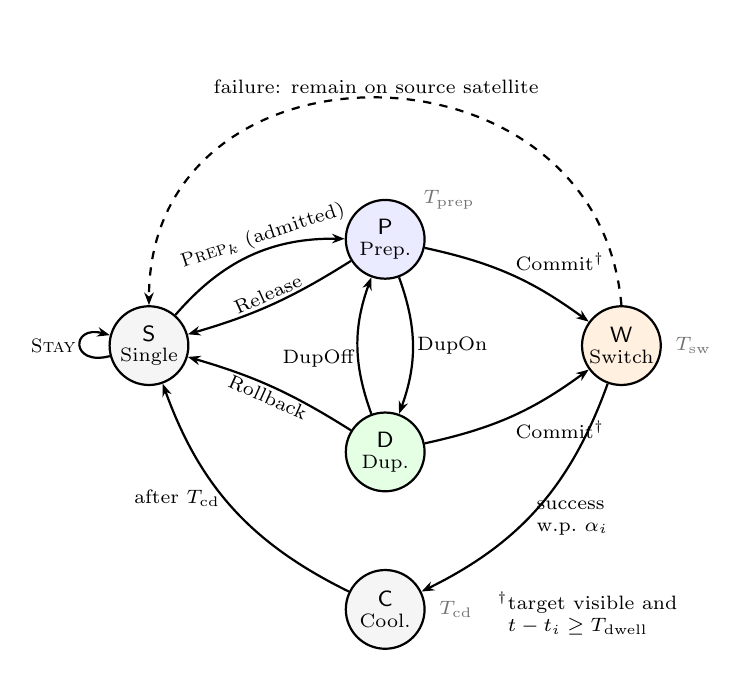
\begin{tikzpicture}[
  >={Stealth[length=1.6mm]}, font=\footnotesize,
  st/.style={circle, draw, thick, minimum size=10mm, inner sep=0pt, align=center},
  tr/.style={->, thick},
  lab/.style={font=\scriptsize, inner sep=1.2pt},
  tm/.style={font=\scriptsize, text=black!55}]
  \node[st, fill=black!4]   (S) at (0,0)       {\textsf{S}\\[-2pt]{\scriptsize Single}};
  \node[st, fill=blue!8]    (P) at (3.0,1.35)  {\textsf{P}\\[-2pt]{\scriptsize Prep.}};
  \node[st, fill=green!10]  (D) at (3.0,-1.35) {\textsf{D}\\[-2pt]{\scriptsize Dup.}};
  \node[st, fill=orange!12] (W) at (6.0,0)     {\textsf{W}\\[-2pt]{\scriptsize Switch}};
  \node[st, fill=black!4]   (C) at (3.0,-3.35) {\textsf{C}\\[-2pt]{\scriptsize Cool.}};
  \node[tm, above right=-1mm and 0mm of P] {$T_{\mathrm{prep}}$};
  \node[tm, right=0.5mm of W] {$T_{\mathrm{sw}}$};
  \node[tm, right=0.5mm of C] {$T_{\mathrm{cd}}$};
  % S <-> P
  \draw[tr] (S) to[bend left=25] node[lab, above, pos=0.6, sloped] {$\textsc{Prep}_k$ (admitted)} (P);
  \draw[tr] (P) to[bend left=8]  node[lab, above, pos=0.5, sloped] {Release} (S);
  % P <-> D
  \draw[tr] (P) to[bend left=20] node[lab, right] {DupOn} (D);
  \draw[tr] (D) to[bend left=20] node[lab, left, pos=0.4] {DupOff} (P);
  % D -> S
  \draw[tr] (D) to[bend right=8] node[lab, below, pos=0.5, sloped] {Rollback} (S);
  % commit
  \draw[tr] (P) to[bend left=12]  node[lab, above right, pos=0.5] {Commit$^{\dagger}$} (W);
  \draw[tr] (D) to[bend right=12] node[lab, below right, pos=0.5] {Commit$^{\dagger}$} (W);
  % outcome of switching
  \draw[tr] (W) to[bend left=22] node[lab, right, align=left, pos=0.55, xshift=0.5mm] {success\\w.p.\ $\alpha_i$} (C);
  \draw[tr] (C) to[bend left=22] node[lab, left, pos=0.55] {after $T_{\mathrm{cd}}$} (S);
  \draw[tr, dashed] (W.north) to[out=95, in=90, looseness=1.5]
        node[lab, above, pos=0.5] {failure: remain on source satellite} (S.north);
  \draw[tr] (S) edge[loop left, looseness=5] node[lab, left] {\textsc{Stay}} (S);
  \node[font=\scriptsize, align=left, anchor=north west] at (4.3,-3.0)
    {$^{\dagger}$target visible and\\ \phantom{$^{\dagger}$}$t-t_i\ge T_{\mathrm{dwell}}$};
\end{tikzpicture}%
}
\caption{Per-UE CHO and PDCP-duplication state machine. $\textsc{Prep}_k$ is
subject to multi-UE admission; the timers $T_{\mathrm{prep}}$,
$T_{\mathrm{sw}}$, and $T_{\mathrm{cd}}$ must elapse before leaving \textsf{P},
\textsf{W}, and \textsf{C}, respectively; a switch succeeds with the
probability~\eqref{eq:hosuccess}. Losing visibility of the target in
\textsf{P} or \textsf{D} also returns the UE to \textsf{S}.}
\label{fig:fsm}
\end{figure}

\subsection{Information Structure and Partial Observability}
\label{sec:obs}

The agents do not observe the complete physical state. Current geometric link
availability is assumed to be known for the serving-link visibility indicator
and candidate presence, whereas radio-quality, elevation, and load information
provided to the actor is delayed by $T_{\mathrm{obs}}$ epochs. In addition,
the observed SINR and load are corrupted by temporally correlated noise.
Specifically,
\begin{gather}
\tilde\gamma_{i\ell}(t)=\gamma_{i\ell}(t-T_{\mathrm{obs}})+\nu_{i\ell}(t),
\label{eq:telemetry}\\
\tilde e_{i\ell}(t)=\min\!\Big\{e_{\max},\max\!\big\{0,\,e_{i\ell}(t-T_{\mathrm{obs}})\,2^{\nu_{i\ell}(t)/10}\big\}\Big\},\notag\\
\tilde\epsilon_{i\ell}(t)=\epsilon_{i\ell}(t-T_{\mathrm{obs}}),\notag\\
\tilde\Phi_{i\ell}(t)=\big[\Phi_\ell(t-1-T_{\mathrm{obs}})+\omega_{i\ell}(t)\big]^+,\notag
\end{gather}
where the telemetry noises $\nu_{i\ell}(t)$ and $\omega_{i\ell}(t)$ are
independent zero-mean AR(1) processes with correlation coefficients
$\rho_\nu$ and $\rho_\omega$ and standard deviations $\sigma_\nu$ and
$\sigma_\omega$, respectively. Thus, elevation telemetry is delayed but is not
subjected to an additional measurement-noise term in the present
implementation. The local observation $\mathbf{o}_i(t)\in\mathbb{R}^{16+7K}$
contains (i) the queue length, head-of-line delay, arrival rate,
reliability-class indicator, duplication flag, one-hot protocol state, and
protocol timer; (ii) for the serving satellite: visibility, $\tilde\gamma$,
$\tilde e$, $\tilde\epsilon$, and $\tilde\Phi$; and (iii) for each candidate:
presence, a prepared-target flag, $\tilde\gamma$, $\tilde e$,
$\tilde\epsilon$, $\tilde\Phi$, and the observed SINR trend
$\tilde\gamma(t)-\tilde\gamma(t-1)$. Agents do \emph{not} observe the
remaining visibility time, the capacity scales, the event realizations, the
latent link regimes, or the states and actions of other UEs. The candidate
list is ranked by observed current SINR only, and the action mask does not
check whether a candidate will remain visible long enough to complete a
handover: anticipating the satellite geometry is left to the decision layer.
The per-UE reliability-class indicator is fixed to $0.99$ in the present
experiments and should not be confused with the system-level outage threshold
$C_{\mathrm{thr}}=0.10$ introduced in Section~\ref{sec:problem}.

\emph{Per-epoch control sequence.}
At decision epoch $t$, UE $i$ forms its local observation from delayed
telemetry, its current protocol state, and its locally experienced history;
in M4 and M5 it additionally receives the satellite congestion prices
computed at the end of the preceding epoch. Each UE then selects one masked
mobility action independently. The environment first resolves ongoing
protocol timers and switching outcomes, re-validates the selected actions
(actions that have become infeasible are replaced by \textsc{Stay}), and
jointly admits the simultaneous preparation requests. New packets arrive,
the fixed scheduler allocates the remaining satellite resources to the
serving and duplicated data legs, and packet delivery, service deficit, and
outage are realized. The resulting local outcomes are fed to the recurrent
memory for the next decision. Finally, the hidden regimes and disturbance
events advance, the links and telemetry are refreshed, and the satellite
coordinator updates its congestion price from the aggregate intended demand,
so that the new price affects only the next decentralized decision.
Coordination is therefore causal and one-epoch delayed rather than based on
instantaneous access to the actions of other UEs.

\subsection{Non-Stationarity: Hidden Regimes and Disturbance Events}
\label{sec:nonstat}

\emph{Hidden link regimes.} Every UE--satellite path $(i,\ell)$ follows a
hidden semi-Markov regime $\textsc{Good}\to\textsc{Degraded}\to\textsc{Recovering}\to\textsc{Good}$.
A path enters \textsc{Degraded} with a small probability per epoch and with a
larger probability at the start of an episode (Table~\ref{tab:params}), stays
there for a duration drawn uniformly between $8$ and $24$ epochs with an extra
loss $Z_{i\ell}$ drawn uniformly between $7$ and $15$\,dB, and then recovers
over $4$ to $10$ epochs, during which $Z_{i\ell}$ decays linearly to zero.
These regimes persist over many epochs and are observable only through their
delayed, noisy effect on $\tilde\gamma$, which is what makes memory useful.

\emph{Disturbance events.} Each training and nominal-evaluation episode
contains five events whose start, duration, severity, affected satellite,
and affected UE subset are sampled from the ranges in Table~\ref{tab:params}:
two blockages (extra loss $B_{i\ell}$ on the selected UE--satellite links),
two capacity drops (reduced capacity scale $\kappa_\ell$ of one satellite),
and one traffic burst (increased arrival rate $\lambda_i$ of a subset of UEs).
For the \emph{compound-stress} evaluation, the randomized training-event
schedule is replaced by a deterministic overlapping disturbance pattern: a
traffic burst with the factor $2.5$ on $50\%$ of the UEs during
$t\in[60,120)$, a capacity drop of satellite $2$ to $45\%$ of its nominal
capacity scale during $t\in[80,130)$, and an $18$-dB blockage affecting all
links of $25\%$ of the UEs during $t\in[100,125)$. The traffic-burst and
blockage severities lie outside their training ranges, and the blockage
affects all satellites of a UE instead of a single one, whereas the
capacity-drop magnitude equals the most severe value of its training range.
More importantly, the three disturbances overlap in time, creating a
compound operating condition not encountered during training.

% ---------------------------------------------------------------------
\begin{table}[t]
\centering
\caption{Simulation and learning parameters}
\label{tab:params}
\footnotesize
\setlength{\tabcolsep}{2pt}
\fitcol{%
\begin{tabular}{@{}ll@{}}
\toprule
\multicolumn{2}{@{}l}{\textbf{Network and protocol}}\\
Satellites / UEs / candidates & $L=6$, $N=12$, $K=3$\\
Altitude, inclination, period & $h=600$\,km, $\iota=53^\circ$, $T_{\mathrm{orb}}=5800$\,s\\
Epoch, episode, min.\ elev. & $\Delta=1$\,s, $T=420$, $\epsilon_{\min}=10^\circ$\\
Carrier, bandwidth & $f=2$\,GHz, $W=4$\,MHz\\
Tx power, Tx/Rx gain & $P_{\mathrm{T}}=46$\,dBm, $G_{\mathrm{T}}=30$\,dBi, $G_{\mathrm{R}}=0$\,dBi\\
Noise figure, interference & $F=7$\,dB, $P_{\mathrm{I}}=-108$\,dBm\\
Losses (atm./impl.) & $A_{\mathrm{atm}}=0.5$\,dB, $A_{\mathrm{impl}}=3$\,dB\\
Shadowing & $\sigma_\chi=2$\,dB, $\rho_\chi=0.95$\\
SE cap, capacity scale & $e_{\max}=6$, $\kappa_0=0.7$\\
Packet size, deadline, queue & $S=12$\,kbit, $T_{\mathrm{dl}}=2$\,s, $Q_{\max}=400$\\
Mean rate, spread & $\bar\lambda=2$\,Mb/s, $\pm35\%$\\
Min.\ service ratio, reliab.\ class & $\beta=0.8$, $0.99$ (all UEs)\\
$T_{\mathrm{prep}},T_{\mathrm{sw}},T_{\mathrm{cd}},T_{\mathrm{dwell}},T_{\mathrm{pp}}$ & $1,2,5,15,20$ epochs\\
Prep.\ reservation, control slots & $\varpi=0.01$, $M=2$\\
HO success, dup.\ corr. & $\alpha_0=0.995$, $\varkappa=0.15$\\
\midrule
\multicolumn{2}{@{}l}{\textbf{Partial observability and non-stationarity}}\\
Telemetry lag & $T_{\mathrm{obs}}=2$ epochs\\
Telemetry noise & $\sigma_\nu=1.5$\,dB, $\sigma_\omega=0.08$, $\rho_\nu=\rho_\omega=0.8$\\
Regime entry probability & $0.06$ (episode start), $0.006$ (per epoch)\\
Blockage (2 events) & $8$--$15$\,dB, $25$--$55$ epochs,\\
 & $30$--$65\%$ of UEs\\
Capacity drop (2 events) & factor $0.45$--$0.80$, $25$--$70$ epochs\\
Traffic burst (1 event) & factor $1.35$--$1.85$, $35$--$70$ epochs\\
\midrule
\multicolumn{2}{@{}l}{\textbf{Objective and agentic modules}}\\
Cost weights & $w=0.25$, $w_{\mathrm{prep}}=0.2$, $w_{\mathrm{HO}}=0.05$\\
Outage threshold & $C_{\mathrm{thr}}=0.10$\\
Dual step size, bound & $\eta_\mu=0.005$, $\mu_{\max}=10$\\
Price step size, bound & $\eta_y=0.05$, $y_{\max}=5$\\
Planning horizon, discount & $\tau_{\max}=6$, $\xi_{\mathrm{p}}=0.95$\\
\midrule
\multicolumn{2}{@{}l}{\textbf{Learning (CTDE-MAPPO)}}\\
Actor / critic MLP & $[128,128]$ / $[256,256]$\\
GRU hidden size, TBPTT length & $128$, $16$\\
Rollout, iterations & $T_{\mathrm{roll}}=128$, $I=2000$\\
PPO epochs, minibatch & $5$, $128$\\
Discount, GAE factor, clip, KL & $\xi=0.99$, $0.95$, $0.2$, $0.03$\\
LR actor/critic & $3{\cdot}10^{-4}\!\to\!3{\cdot}10^{-5}$ / $10^{-3}\!\to\!10^{-4}$\\
Entropy / value coef., grad.\ norm & $0.01$ / $0.5$, $0.5$\\
\bottomrule
\end{tabular}%
}
\end{table}
% ---------------------------------------------------------------------

% =====================================================================
\section{Problem Formulation}
\label{sec:problem}
% =====================================================================

\subsection{Per-Epoch Costs}

Let $\Nset(t)\subseteq\Nset$ be the set of UEs that are active in epoch $t$.
We define the service, control, and reliability costs of epoch $t$ as
\begin{align}
C_{\mathrm{def}}(t) &= \frac{1}{|\Nset(t)|}\sum_{i\in\Nset(t)}\delta_i(t),\\
C_{\mathrm{prep}}(t) &= \frac{\varpi}{L}\sum_{\ell\in\Lset}n_\ell(t),\\
C_{\mathrm{HO}}(t) &= \frac{1}{|\Nset(t)|}\sum_{i\in\Nset(t)}\ind\{a_i(t)=\textsc{Commit}\},\\
C_{\mathrm{ctrl}}(t) &= C_{\mathrm{dup}}(t)+w_{\mathrm{prep}}C_{\mathrm{prep}}(t)+w_{\mathrm{HO}}C_{\mathrm{HO}}(t),\\
C_{\mathrm{out}}(t) &= \frac{1}{|\Nset(t)|}\sum_{i\in\Nset(t)}u_i(t),
\end{align}
where the duplication cost $C_{\mathrm{dup}}(t)$ is the fraction of the bits
scheduled for transmission in epoch $t$ that are duplicate copies sent over
secondary legs. Hence, $C_{\mathrm{dup}}$ measures transmission redundancy
rather than successfully delivered traffic. The control cost
$C_{\mathrm{ctrl}}$ is a resource- and mobility-control-cost proxy comprising
duplicated transmissions, target preparation reservations, and handover
executions with the weights $w_{\mathrm{prep}}$ and $w_{\mathrm{HO}}$. It does
not explicitly charge the number of preparation signalling messages; this
distinction is revisited in Section~\ref{sec:limitations}.

\subsection{Constrained Decentralized POMDP}

The problem is a cooperative, constrained decentralized partially observable
Markov decision process (Dec-POMDP) with the agent set $\Nset$, the state
space $\mathcal{S}$, the action set $\Aset$ of every agent, the transition
kernel $\mathcal{P}$, the team reward $r$, and the discount factor $\xi$. The
state $s(t)\in\mathcal{S}$ comprises the satellite geometry, channel and
shadowing states, hidden regimes, event realizations, queues, and protocol
states of all UEs; $\mathcal{P}$ is given by Section~\ref{sec:system}; and
each agent receives the local observation $\mathbf{o}_i(t)$ of
Section~\ref{sec:obs} together with its action mask. All agents share the team
reward
\begin{equation}
r(t) = -C_{\mathrm{def}}(t) - w\,C_{\mathrm{ctrl}}(t),
\label{eq:reward}
\end{equation}
where $w$ weights the control cost against the service deficit. Reliability
is imposed as a constraint on the long-run outage cost rather than as a
further reward weight:
\begin{equation}
\max_{\boldsymbol\pi}\ \E_{\boldsymbol\pi}\Big[\sum_{t}\xi^t r(t)\Big]
\ \ \text{s.t.}\ \ \E_{\boldsymbol\pi}\big[C_{\mathrm{out}}(t)\big]\le C_{\mathrm{thr}},
\label{eq:cdecpomdp}
\end{equation}
where $C_{\mathrm{thr}}$ is the outage threshold and
$\boldsymbol\pi=(\pi_1,\dots,\pi_N)$ are decentralized policies that map the
local observation history of each UE to its action. The per-satellite
capacity constraints are enforced by the scheduler and the admission rule and
need not be learned. Problem~\eqref{eq:cdecpomdp} is solved through its
Lagrangian relaxation
\begin{gather}
\max_{\boldsymbol\pi}\min_{\mu\ge0}\ \E_{\boldsymbol\pi}\Big[\sum_t\xi^t r_\mu(t)\Big],\label{eq:lagrangian}\\
r_\mu(t)=r(t)-\mu\big(C_{\mathrm{out}}(t)-C_{\mathrm{thr}}\big),\notag
\end{gather}
where $\mu$ is the reliability multiplier.

\emph{Why the problem is hard.} Three features make \eqref{eq:cdecpomdp}
difficult for conventional CHO rules and for memoryless learning:
(i) \emph{partial observability} with delayed, noisy telemetry and hidden,
persistent link regimes; (ii) \emph{delayed consequences}: a preparation
blocks resources and control slots before any benefit appears, the dwell guard
restricts future switches, and a target chosen now may set before the switch
completes; and (iii) \emph{coupling}: UEs compete for preparation slots,
reservations, and data capacity, and congestion lowers the handover success
probability \eqref{eq:hosuccess}.

% =====================================================================
\section{Proposed Capability-Structured Agentic Framework}
\label{sec:method}
% =====================================================================

We operationalize agentic control through a structured set of
capabilities rather than treating agentic AI as synonymous with an
LLM-based controller. The architecture combines a learned decentralized
policy with lightweight domain-specific mechanisms that exploit the structure
of LEO mobility, following the four capabilities of agentic AI.
\emph{Perception} is provided by masked, telemetry-based local observation and
per-UE autonomous action selection; \emph{memory} by a recurrent state that
infers persistent hidden conditions from delayed feedback; \emph{reasoning} by
a protocol-aware ephemeris lookahead that anticipates the delayed
consequences of preparation and switching; and \emph{coordination} by a
low-dimensional satellite congestion price that summarizes shared-resource
pressure without exchanging UE actions. Finally, a training-time reliability
multiplier provides explicit \emph{goal regulation}.

These capabilities are introduced incrementally to form the M1--M5 model
family in Table~\ref{tab:models}; Fig.~\ref{fig:arch} shows the resulting
agent. The resulting ladder is an architectural decomposition used for
capability-structured evaluation, not an assumption that performance must
improve monotonically from M1 to M5. Each variant is trained independently in
the same environment with the same base reward, except for the reliability
Lagrangian used by M5. No language model is required, and online execution
remains numerical and lightweight: actions are produced locally by each UE,
while satellites broadcast only the scalar congestion prices required by M4
and M5.

\begin{table}[t]
\centering
\caption{Capability-structured model family}
\label{tab:models}
\footnotesize
\setlength{\tabcolsep}{2.5pt}
\fitcol{%
\begin{tabular}{@{}lllll@{}}
\toprule
Model & Capability added & Actor input $\mathbf{z}_i$ & Training reward\\
\midrule
M1 & Perception (core) & $\mathbf{o}_i$ & $r$\\
M2 & + Memory & $[\mathbf{o}_i,\mathbf{g}_i]$ & $r$\\
M3 & + Reasoning & $[\mathbf{o}_i,\mathbf{g}_i,\boldsymbol\phi_i]$ & $r$\\
M4 & + Coordination & $[\mathbf{o}_i,\mathbf{g}_i,\boldsymbol\phi_i,\mathbf{y}_i/y_{\max}]$ & $r$\\
M5 & + Goal regulation & $[\mathbf{o}_i,\mathbf{g}_i,\boldsymbol\phi_i,\mathbf{y}_i/y_{\max},\mu/\mu_{\max}]$ & $r_\mu$\\
\bottomrule
\end{tabular}%
}
\end{table}

\begin{figure*}[t]
\centering
\resizebox{\textwidth}{!}{%
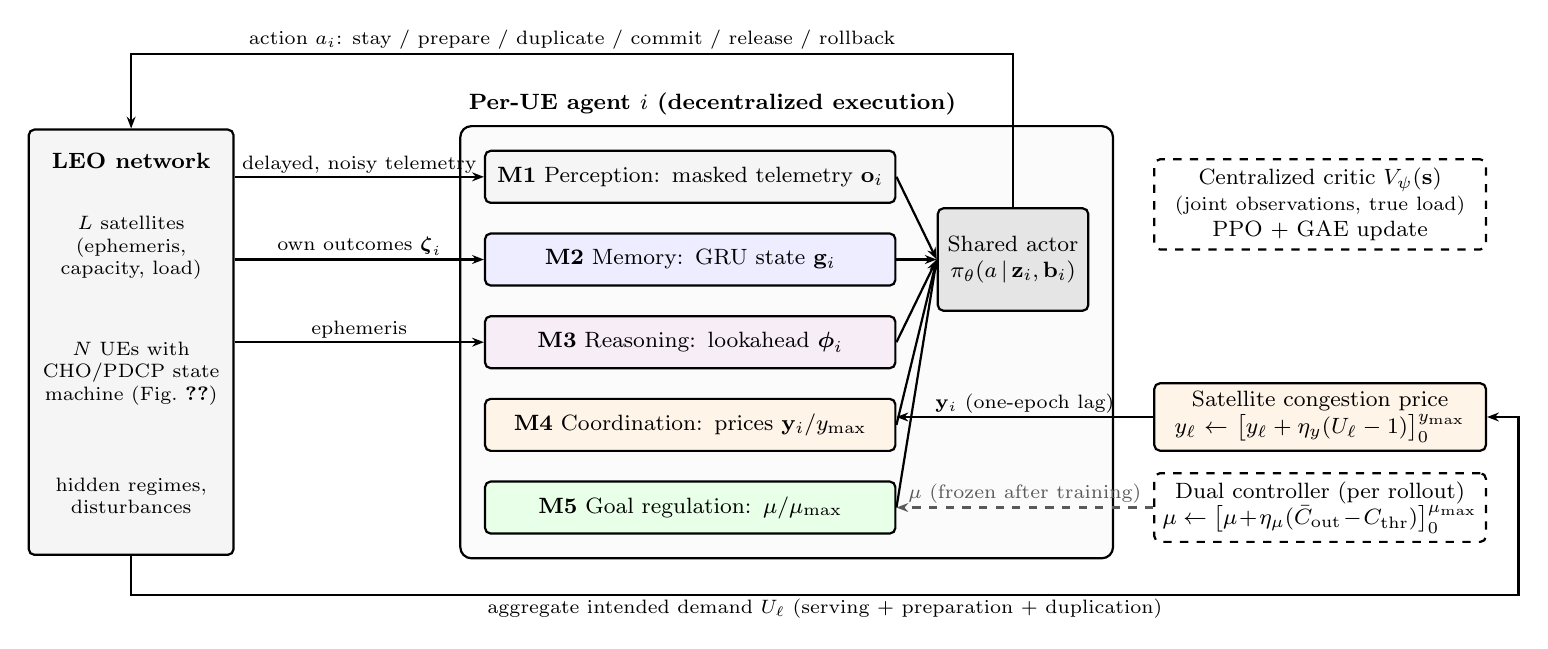
\begin{tikzpicture}[
  >={Stealth[length=1.5mm]}, font=\footnotesize,
  box/.style={draw, thick, rounded corners=2pt, align=center, inner sep=3pt},
  mod/.style={box, text width=5.0cm, minimum height=0.66cm, fill=#1},
  rbox/.style={box, text width=4.0cm},
  ar/.style={->, thick},
  tra/.style={->, thick, dashed, black!65},
  lab/.style={font=\scriptsize, inner sep=1pt}]
  % ---------------- environment ----------------
  \node[box, fill=black!4, minimum width=2.6cm, minimum height=5.4cm] (env) at (0,0) {};
  \node[font=\footnotesize\bfseries] at (0,2.3) {LEO network};
  \node[align=center, font=\scriptsize] at (0,1.2) {$L$ satellites\\(ephemeris,\\capacity, load)};
  \node[align=center, font=\scriptsize] at (0,-0.4) {$N$ UEs with\\CHO/PDCP state\\machine (Fig.~\ref{fig:fsm})};
  \node[align=center, font=\scriptsize] at (0,-1.95) {hidden regimes,\\disturbances};
  % ---------------- per-UE agent ----------------
  \node[mod=black!4]  (per) at (7.1, 2.1)  {\textbf{M1} Perception: masked telemetry $\mathbf{o}_i$};
  \node[mod=blue!7]   (mem) at (7.1, 1.05) {\textbf{M2} Memory: GRU state $\mathbf{g}_i$};
  \node[mod=violet!7] (rea) at (7.1, 0.0)  {\textbf{M3} Reasoning: lookahead $\boldsymbol\phi_i$};
  \node[mod=orange!9] (coo) at (7.1,-1.05) {\textbf{M4} Coordination: prices $\mathbf{y}_i/y_{\max}$};
  \node[mod=green!9]  (goa) at (7.1,-2.1)  {\textbf{M5} Goal regulation: $\mu/\mu_{\max}$};
  \node[box, fill=black!10, text width=1.7cm, minimum height=1.3cm] (act) at (11.2,1.05)
       {Shared actor\\$\pi_\theta(a\,|\,\mathbf{z}_i,\mathbf{b}_i)$};
  \foreach \n in {per, mem, rea, coo, goa} \draw[ar] (\n.east) -- (act.west);
  \begin{scope}[on background layer]
    \node[draw, thick, rounded corners=4pt, fill=black!1.5, fit=(per)(goa)(act),
          inner xsep=3mm, inner ysep=3mm] (agent) {};
  \end{scope}
  \node[font=\footnotesize\bfseries, anchor=south west] at (agent.north west) {Per-UE agent $i$ (decentralized execution)};
  % ---------------- right column ----------------
  \node[rbox, dashed, fill=white] (crit) at (15.1, 1.75)
       {Centralized critic $V_\psi(\mathbf{s})$\\{\scriptsize (joint observations, true load)}\\PPO + GAE update};
  \node[rbox, fill=orange!9] (price) at (15.1,-0.95)
       {Satellite congestion price\\$y_\ell\leftarrow\big[y_\ell+\eta_y(U_\ell-1)\big]_0^{y_{\max}}$};
  \node[rbox, dashed, fill=white] (dual) at (15.1,-2.1)
       {Dual controller (per rollout)\\$\mu\leftarrow\big[\mu+\eta_\mu(\bar C_{\mathrm{out}}-C_{\mathrm{thr}})\big]_0^{\mu_{\max}}$};
  % ---------------- arrows ----------------
  \draw[ar] (env.east |- per) -- node[lab, above] {delayed, noisy telemetry} (per.west);
  \draw[ar] (env.east |- mem) -- node[lab, above] {own outcomes $\boldsymbol\zeta_i$} (mem.west);
  \draw[ar] (env.east |- rea) -- node[lab, above] {ephemeris} (rea.west);
  \draw[ar] (price.west) -- node[lab, above] {$\mathbf{y}_i$ (one-epoch lag)} (price.west -| coo.east);
  \draw[tra] (dual.west) -- node[lab, above] {$\mu$ (frozen after training)} (dual.west -| goa.east);
  \draw[ar] (act.north) -- ++(0,1.95) -| node[lab, above, pos=0.25]
        {action $a_i$: stay / prepare / duplicate / commit / release / rollback} (env.north);
  \draw[ar] (env.south) -- ++(0,-0.5) -| node[lab, below, pos=0.25]
        {aggregate intended demand $U_\ell$ (serving + preparation + duplication)} ($(price.east)+(0.4,0)$) -- (price.east);
\end{tikzpicture}%
}
\caption{Architecture of the capability-structured agent. Each UE runs the
same actor on the concatenation $\mathbf{z}_i$ of the capability outputs
available in its variant (M1: $\mathbf{o}_i$; M2 adds $\mathbf{g}_i$; M3 adds
$\boldsymbol\phi_i$; M4 adds $\mathbf{y}_i/y_{\max}$; M5 adds $\mu/\mu_{\max}$).
Solid: execution; dashed: training only. Satellites broadcast only the scalar
prices.}
\label{fig:arch}
\end{figure*}

\subsection{Perception and Core Decision Making (M1)}

All UEs share one stochastic actor $\pi_\theta$ with parameters $\theta$ and
are trained with centralized training and decentralized execution (CTDE)
using multi-agent proximal policy optimization (MAPPO)~\cite{yu2022mappo}. The
actor maps its input $\mathbf{z}_i(t)$ to one logit per action through a
neural network $\mathrm{NN}_\theta$, and invalid actions are removed by a
masked softmax,
\begin{equation}
\pi_\theta(a\mid\mathbf{z}_i,\mathbf{b}_i)=\frac{b_{i,a}\exp\big([\mathrm{NN}_\theta(\mathbf{z}_i)]_a\big)}{\mathbf{b}_i^{\mathsf T}\exp\big(\mathrm{NN}_\theta(\mathbf{z}_i)\big)},
\end{equation}
where $b_{i,a}$ is the entry of $\mathbf{b}_i$ for action $a$ and the
exponential in the denominator is applied elementwise. Perception in M1 is
the masked, telemetry-based observation $\mathbf{z}_i=\mathbf{o}_i$. The
centralized critic $V_\psi$ with parameters $\psi$ is used only during
training. Its input $\mathbf{s}(t)$ concatenates the observations of all UEs
with the true per-satellite utilization and pressure $\Phi_\ell$, and, when
available, the satellite prices and the reliability multiplier.

\subsection{Memory: Inferring Hidden Regimes (M2)}

Because link regimes are hidden and telemetry is delayed, the current
observation is not a sufficient statistic. M2 equips every agent with a gated
recurrent unit (GRU) that summarizes its interaction history in the recurrent
memory
\begin{equation}
\mathbf{g}_i(t)=\mathrm{GRU}_\theta\big(\mathbf{g}_i(t-1),\ [\mathbf{o}_i(t),\ \mathrm{onehot}(a_i(t-1)),\ \boldsymbol\zeta_i(t-1)]\big),
\end{equation}
where $\boldsymbol\zeta_i\in\mathbb{R}^6$ is the agent's own \emph{experienced
outcome}: the last handover result ($+1$ success, $-1$ failure, $0$ none), its
outage indicator $u_i$, its deficit $\delta_i$, the duplication gain (the part
of its expected goodput contributed by the secondary leg, normalized by
$D_i$), its resource-usage indicator, and the experienced congestion
$\Phi/(1+\Phi)$ of its serving or target satellite. The actor input becomes
$\mathbf{z}_i=[\mathbf{o}_i,\mathbf{g}_i]$. Memory thus supports long-horizon
adaptation to non-stationary link conditions using only locally available
feedback. The GRU is trained end-to-end with truncated backpropagation through
time.

\subsection{Reasoning: Protocol-Aware Ephemeris Lookahead (M3)}

The mask does not prevent choosing a target that is about to set, and the
benefit of a preparation appears only several epochs later. M3 therefore adds
an analytical planner that exploits the one piece of information that is
deterministic in LEO systems: the satellite ephemeris. For every feasible
first action $a$, the planner evaluates a small library $\mathcal{Q}_i(a)$ of
protocol-consistent plans, i.e., action sequences
$\mathbf{a}=(a(0),\dots,a(\tau_{\max}-1))$ of length $\tau_{\max}$ that start
with $a$ (e.g., $\textsc{Prep}_k$--wait--$\textsc{Commit}$;
$\textsc{Prep}_k$--wait--$\textsc{DupOn}$--$\textsc{Commit}$; $\textsc{Stay}$)
and are padded with $\textsc{Stay}$, by rolling the UE's own protocol state
machine forward. For tractability, this hypothetical rollout propagates
protocol timers deterministically. Once a hypothetical \textsc{Commit}
satisfies the dwell and predicted-visibility conditions, completion of the
corresponding switch is treated as successful in the lookahead. Consequently,
the stochastic handover-success model in \eqref{eq:hosuccess} is realized by
the environment but is not explicitly sampled or averaged inside the
analytical planner.

The SINR of link $(i,\ell)$ at the lookahead step
$\tau\in\{0,\dots,\tau_{\max}-1\}$ is predicted from the \emph{observed} SINR
and the ephemeris-predicted range,
\begin{equation}
\hat\gamma_{i\ell}(t+\tau)=\tilde\gamma_{i\ell}(t)-20\log_{10}\frac{d_{i\ell}(t+\tau)}{d_{i\ell}(t)},
\end{equation}
and the link is treated as unavailable once $\epsilon_{i\ell}(t+\tau)<\epsilon_{\min}$.
The predicted leg rate uses the nominal capacity scale $\kappa_0$ scaled by the
observed load $\tilde\Phi_{i\ell}$, from which the planner obtains the
predicted deficit $\hat\delta_i(t+\tau\mid\mathbf{a})$ under plan
$\mathbf{a}$, including the duplication diversity of \eqref{eq:dup}. The cost
of a first action is the best discounted plan cost,
\begin{multline}
J_i(a)=\min_{\mathbf{a}\in\mathcal{Q}_i(a)}\sum_{\tau=0}^{\tau_{\max}-1}\xi_{\mathrm{p}}^\tau\Big(\hat\delta_i(t+\tau\mid\mathbf{a})\\
+\mathbf{y}(t)^{\mathsf T}\big[\hat{\mathbf{x}}_i(t+\tau\mid\mathbf{a})-\hat{\mathbf{x}}_i(t+\tau\mid\mathbf{a}_0)\big]^+\Big),
\label{eq:plancost}
\end{multline}
where $\xi_{\mathrm{p}}$ is the planning discount, $\mathbf{a}_0$ is the plan
that stays throughout, and the second term is present only in M4 and M5. Here,
$\mathbf{y}(t)=[y_1(t),\ldots,y_L(t)]^{\mathsf T}$ denotes the \emph{raw}
satellite-price vector maintained by the coordinator. Only entries
corresponding to the UE's serving and hypothetical target satellites contribute
to the inner product.

The vector $\hat{\mathbf{x}}_i$ represents the planner's predicted
per-satellite resource footprint of UE $i$. In the present implementation it
contains the predicted serving-leg resource fraction, the secondary-leg
resource fraction while duplicating, and the data-plane reservation $\varpi$
while a target reservation is active. The positive-part difference with the
footprint of $\mathbf{a}_0$ therefore prices only the incremental resource
footprint relative to remaining with the current serving satellite.

Importantly, $\hat{\mathbf{x}}_i$ is not identical to the aggregate intended
demand $U_\ell$ used by the satellite coordinator (Section~\ref{sec:coord}).
The control-plane preparation-contention term $m_\ell/M$ is included in
$U_\ell$ when the satellite price is updated, but is not explicitly inserted
into the single-UE hypothetical footprint. Its effect therefore reaches the
reasoner indirectly through the broadcast congestion price.

The reasoner deliberately ranks plans primarily by predicted service
continuity rather than reproducing the complete MAPPO training reward. In M3,
the second term of \eqref{eq:plancost} is absent, so resource and
mobility-control costs are learned through the team reward rather than
hard-coded into the planner. M4 and M5 add the marginal raw-price term,
allowing the same geometry-aware lookahead to account for recently observed
shared resource pressure.

Let $J_{\min}$ and $J_{\max}$ be the minimum and maximum of $J_i(a)$ over the
feasible actions of UE $i$. The reasoning feature of a feasible action is
\begin{equation}
\phi_{i,a}=
\begin{cases}
\dfrac{J_i(a)-J_{\min}}{J_{\max}-J_{\min}}, & J_{\max}-J_{\min}>10^{-8},\\[6pt]
0, & \text{otherwise},
\end{cases}
\label{eq:reasoning_feature}
\end{equation}
and $\phi_{i,a}=1$ for masked actions. The vector
$\boldsymbol\phi_i\in[0,1]^{K+6}$ is appended to the actor input:
$\mathbf{z}_i=[\mathbf{o}_i,\mathbf{g}_i,\boldsymbol\phi_i]$. The planner is
\emph{advisory}: the actor learns how much to trust it. It has no access to
future events, hidden regimes, true capacity scales, or the states of other
UEs.

\subsection{Coordination: Congestion Prices (M4)}
\label{sec:coord}

UEs compete for preparation slots, reservations, and data capacity, but
exchanging intentions between UEs is impractical. M4 coordinates them through
a lightweight price signal maintained by each satellite. Let $\mathcal{D}(t)$
be the set of UEs that duplicate in epoch $t$. Satellite $\ell$ measures its
aggregate intended demand
\begin{equation}
U_\ell(t)=\sum_{i:\,\ell_i(t)=\ell}x_{i\ell}(t)+\frac{m_\ell(t)}{M}+\sum_{i\in\mathcal{D}(t):\,c_i(t)=\ell}x_{i\ell}(t),
\end{equation}
i.e., the serving demand, the new preparation requests normalized by the
number of control slots, and the duplication demand, and updates its price
$y_\ell$ by projected subgradient ascent with the step size $\eta_y$,
\begin{equation}
y_\ell(t+1)=\Big[y_\ell(t)+\eta_y\big(U_\ell(t)-1\big)\Big]_0^{y_{\max}}.
\label{eq:price}
\end{equation}
Prices rise while intended demand exceeds the normalized resource level and
decay otherwise; they are reset at the start of each episode and are not
learned. The price produced at the end of epoch $t$ is used only for the next
decentralized decision, so coordination is causal and one-epoch delayed.

The actor of UE $i$ receives the local price vector
$\mathbf{y}_i(t)=[y_\ell(t)]_{\ell\in\{\ell_i(t)\}\cup\mathcal{K}_i(t)}$ of its
serving satellite and its $K$ candidates, normalized as
$\mathbf{y}_i(t)/y_{\max}$ to provide a bounded neural-network input. In
contrast, the analytical lookahead in \eqref{eq:plancost} uses the raw prices,
which directly weight the planner's incremental resource demand.

The coordinator never allocates actions: decisions remain decentralized, and
the signalling required for coordination is one scalar price per satellite and
control epoch. The price should therefore be interpreted as compressed
coordination context rather than a centralized allocation command. It reveals
neither individual UE states, actions, queues, nor future events, and conveys
only the recent aggregate resource pressure seen by each satellite.

\subsection{Goal Regulation: Primal--Dual Reliability Control (M5)}

M5 addresses the Lagrangian problem~\eqref{eq:lagrangian}. The dual update
uses the realized outage fraction over all active-UE opportunities in one
rollout. For the set $\mathcal{T}$ of the $T_{\mathrm{roll}}$ epochs of a
rollout, the implementation computes the rollout-average outage cost
\begin{equation}
\bar C_{\mathrm{out}}=
\frac{\sum_{t\in\mathcal{T}}\sum_{i\in\Nset(t)}u_i(t)}{\sum_{t\in\mathcal{T}}|\Nset(t)|}.
\end{equation}
After every rollout, the multiplier is updated by the projected step
\begin{equation}
\mu\leftarrow\Big[\mu+\eta_\mu\big(\bar C_{\mathrm{out}}-C_{\mathrm{thr}}\big)\Big]_0^{\mu_{\max}},
\label{eq:dual}
\end{equation}
and the policy is trained on $r_\mu$. The multiplier is held fixed within
each rollout, updated between policy iterations, and frozen after training.
In our implementation, $\mu$ does not modify the ranking of the analytical
lookahead; reliability enters the learned decision through the Lagrangian
reward, the recurrently observed outcomes, and the normalized feature
$\mu/\mu_{\max}$ supplied to the actor and the critic. Consequently, $\mu=0$
makes the \emph{instantaneous training reward} identical to the M4 base
reward, but a trained M5 network remains a separately optimized policy and is
not identical to M4.
% [확인] 평가 시 mu를 바꿔도 행동이 거의 변하지 않았습니다(mu sensitivity 결과).

\subsection{Training Procedure and Complexity}

Algorithm~\ref{alg:train} summarizes training. The shared actor and the
centralized critic are optimized with the clipped PPO
objective~\cite{schulman2017ppo} and generalized advantage
estimation~\cite{schulman2016gae} on the team reward ($r$ or $r_\mu$), with
early stopping at a target KL divergence and linearly annealed learning rates.

\begin{algorithm}[t]
\caption{Training of the capability-structured agents}
\label{alg:train}
\begin{algorithmic}[1]
\State Initialize $\theta$ (actor, GRU), $\psi$ (critic), $\mu\gets0$
\For{iteration $=1,\dots,I$}
  \For{each epoch $t\in\mathcal{T}$ of the rollout}
    \State Each UE forms $\mathbf{o}_i(t)$ and $\mathbf{b}_i(t)$ \Comment{perception}
    \State $\mathbf{g}_i(t)\gets\mathrm{GRU}_\theta(\cdot)$ \Comment{M2+}
    \State $\boldsymbol\phi_i(t)\gets$ lookahead \eqref{eq:plancost} with $\mathbf{y}(t)$ \Comment{M3+}
    \State $a_i(t)\sim\pi_\theta(\cdot\mid\mathbf{z}_i(t),\mathbf{b}_i(t))$ for all $i$ in parallel
    \State Environment step; observe $r(t)$, $C_{\mathrm{out}}(t)$, $\boldsymbol\zeta_i(t)$
    \State Satellites update prices by \eqref{eq:price} \Comment{M4+}
  \EndFor
  \State Compute $r_\mu$ with the current $\mu$ \Comment{M5}
  \State Update $\theta,\psi$ with PPO, GAE, and TBPTT
  \State Update $\mu$ by \eqref{eq:dual} \Comment{M5}
\EndFor
\end{algorithmic}
\end{algorithm}

\emph{Execution complexity.} In each control epoch, a UE performs one
recurrent-state update and one actor forward pass. For M3--M5, the analytical
reasoner evaluates at most $\max\{2K+1,4\}$ protocol-consistent plans, each
over $\tau_{\max}$ epochs. Its per-agent planning complexity is therefore
$\mathcal{O}(K\tau_{\max})$ and does not grow with the total number of UEs.
Across all $N$ agents, the aggregate reasoning work is
$\mathcal{O}(NK\tau_{\max})$, but the $N$ per-UE computations are mutually
independent and can be executed in parallel. Coordination requires only one
congestion price per satellite and epoch, and the M5 reliability multiplier
introduces no execution-time inter-UE signalling.
Measured on a single CPU thread of a desktop processor with an unoptimized
Python/NumPy implementation, the mean actor inference time per epoch for all
$N=12$ UEs is $0.24$--$0.44$\,ms, and the analytical reasoner adds
$19.6$--$21.3$\,ms. The total mean decision latency of M3--M5 is thus at
most $21.7$\,ms, i.e., about $1.8$\,ms per UE, which is more than an order of
magnitude below the $\Delta=1$\,s control epoch.
% [확인] CPU 모델명을 넣으세요 (예: Intel Core i7-12700).

% =====================================================================
\section{Simulation Setup}
\label{sec:setup}
% =====================================================================

\subsection{Training}
All variants use the environment and parameters of Table~\ref{tab:params}.
Each variant is trained for $I=2000$ iterations with five independent
training seeds $\{7,8,9,10,11\}$; the seed determines both the network
initialization and the training-environment realization. The five M1--M5
variants therefore comprise $25$ independently trained policies. Training
episodes contain the randomized disturbance schedule of
Section~\ref{sec:nonstat}; the compound-stress pattern is never used for
training. To isolate goal regulation from the other capabilities, we
additionally train an ablation variant, denoted M1D, which is the memoryless
M1 trained with the Lagrangian reward $r_\mu$ and the same dual controller as
M5, using the same five seeds. The actor input of M1D is unchanged, and $\mu$
enters only its critic. M1D is not part of the capability ladder.

\subsection{Evaluation Protocol}
Every trained policy is evaluated on five held-out evaluation seeds with
$40$ episodes each, under two conditions: \emph{nominal} (randomized events
drawn as in training) and \emph{compound stress}
(Section~\ref{sec:nonstat}). The episode streams of different evaluation
seeds are disjoint, and all methods are evaluated on identical episode
streams, which yields paired comparisons. Actions are sampled from the
stochastic policies; congestion prices evolve online and are reset at the
start of each episode, and the multiplier of M5 is frozen at its trained
value. For a learned variant, each training seed is first averaged over the
five evaluation seeds, and the mean and the Student-$t$ $95\%$ confidence
interval (CI) are computed across the five training seeds, so the CI
reflects training variability. Differences between learned variants are
tested with Welch's $t$-test on the five per-seed means, and
``significant'' refers to the $5\%$ level. Rule-based baselines have no training seed;
their CI is computed across the evaluation seeds and mainly reflects the
difficulty of the individual scenarios. Besides the realized outage ratio,
we report the service deficit, the number of handover executions per epoch
(summed over the $N$ UEs), the ping-pong ratio (ping-pongs per successful
handover), the resource cost $C_{\mathrm{ctrl}}=C_{\mathrm{dup}}+w_{\mathrm{prep}}C_{\mathrm{prep}}+w_{\mathrm{HO}}C_{\mathrm{HO}}$,
and the \emph{common reward} $r=-C_{\mathrm{def}}-w C_{\mathrm{ctrl}}$
of~\eqref{eq:reward}. The common reward is used for all methods, including
M5, whose training reward additionally contains the Lagrangian term.
Two within-policy ablations are evaluated on the same episodes: forcing the
congestion price to zero (M4 and M5), and replacing the reasoning feature by an
uninformative one (M3--M5), i.e., $\phi_{i,a}=0$ for every feasible action and
$\phi_{i,a}=1$ for every masked action, which is the value the actor observes
during training whenever all plan costs are tied.
% [확인] resource cost = C_ctrl (control cost)입니다. 표의 "Resource"와 common reward의 C_ctrl가 같은 양입니다.

\subsection{Baselines}
All baselines observe the same delayed and noisy telemetry and are subject
to the same action masks and admission rules as the learned agents.
\begin{itemize}
\item \emph{CHO (A3/TTT)}: a 3GPP-inspired conditional handover. The best
observed candidate is prepared when it exceeds the serving satellite by
$1$\,dB; the prepared target is executed when it exceeds the serving
satellite by an execution offset for a number of consecutive epochs given by
the time-to-trigger (TTT), and it is released after it falls below the
serving satellite by $1$\,dB for three epochs. The execution offset
($2$, $3$, or $4$\,dB) and the TTT ($1$, $2$, or $3$ epochs) were tuned for
the common reward on three validation seeds whose episodes are disjoint from
all evaluation episodes, and then frozen at $2$\,dB and one epoch. The
selected offset is the smallest value of the grid, and a TTT of one epoch is
the smallest feasible value at $\Delta=1$\,s.
\item \emph{CHO (A3/TTT)+Dup}: the tuned CHO rule, additionally activating
duplication while a target is prepared and the serving SINR is below a
threshold tuned in the same way ($6$\,dB, selected from $\{2,4,6\}$\,dB).
\item \emph{Max-SINR}: prepares the best observed candidate when it exceeds
the serving satellite by $1$\,dB and executes as soon as allowed, without
duplication.
\item \emph{Always-Dup}: always prepares the best observed candidate,
activates duplication, and executes.
\item \emph{Threshold-Dup}: prepares the best candidate when the serving SINR
falls below $4$\,dB, activates duplication, and executes when the target
exceeds the serving satellite by $1$\,dB.
\end{itemize}
Learning-based handover schemes from the literature
\cite{yang2023dqn,liu2024marlho,yang2024fingerprints,zhao2026hrl} select a
serving satellite or trigger a handover, but they do not expose preparation,
duplication, release, and rollback actions and therefore cannot be applied
to the considered action space without redesign. As the learned reference, we
therefore use M1, a CTDE-MAPPO policy~\cite{yu2022mappo} trained on the same
observation space, action space, and reward as the proposed agents but
without any of the agentic extensions; it is denoted MAPPO (M1) in the
comparisons.

% =====================================================================
\section{Results}
\label{sec:results}
% =====================================================================

\begin{figure}[t]
\centering
\figinclude{fig/pdf/fig01_training.pdf}
\caption{Training convergence in terms of the common reward
$r=-C_{\mathrm{def}}-w C_{\mathrm{ctrl}}$ (moving average over $50$
iterations, mean over five training seeds). M5 and M1D are trained on the
Lagrangian reward $r_\mu$ but are shown with the common reward for
comparability.}
\label{fig:training}
\end{figure}

\subsection{Training Convergence}
Fig.~\ref{fig:training} shows the common reward during training. All
variants improve from approximately $-0.13$ to $-0.07$ within the first few
hundred iterations and then refine slowly under the annealed learning rates.
Averaged over the last $100$ iterations, M1 attains the highest training common
reward ($-0.067$), M2, M4, and M5 reach about $-0.072$, and M3 reaches $-0.075$;
this ordering mirrors the common reward on the held-out scenarios
(Table~\ref{tab:main}). M5 is not trained on the common reward but on the
Lagrangian reward $r_\mu$, whose logged value additionally contains the
reliability penalty $\mu(C_{\mathrm{out}}-C_{\mathrm{thr}})$ and is
therefore not comparable across variants; in terms of the common reward, M5
is on par with M2 and M4 while being markedly more efficient in mobility and
resource usage. Because each training seed also defines a different
training-environment realization, the curves are compared qualitatively, and
the variants are compared quantitatively only on the common held-out
evaluation scenarios.

\begin{table*}[t]
\centering
\caption{Performance under nominal and compound-stress conditions (mean $\pm$ 95\% CI half-width). Learned models: CI across $5$ independently trained policies, each evaluated on $5$ evaluation seeds $\times$ $40$ episodes. Heuristics: CI across the $5$ evaluation seeds. HO executions are counted per control epoch over all $N=12$ UEs; the ping-pong ratio is relative to successful handovers; common reward $r=-C_{\mathrm{def}}-w C_{\mathrm{ctrl}}$. Bold: best value in each column and condition; underlined: best learned variant where a rule-based scheme is best; shaded: full agentic stack (M5). Threshold-Dup attains the lowest handover counts only because it rarely hands over, at the cost of the highest outage.}
\label{tab:main}
\footnotesize
\setlength{\tabcolsep}{4pt}
\begin{tabular}{@{}llcccccc@{}}
\toprule
 & Method & Outage $\downarrow$ & Deficit $\downarrow$ & HO exec./epoch $\downarrow$ & Ping-pong $\downarrow$ & Resource ($\times10^{-3}$) $\downarrow$ & Common reward $\uparrow$\\
\midrule
\multirow{10}{*}{\rotatebox{90}{Nominal}} & M1 & $\mathbf{0.131}\,{\pm}\,\mathbf{0.008}$ & $\mathbf{0.065}\,{\pm}\,\mathbf{0.004}$ & $0.367\,{\pm}\,0.082$ & $0.118\,{\pm}\,0.028$ & $5.48\,{\pm}\,2.11$ & $\mathbf{-0.066}\,{\pm}\,\mathbf{0.005}$\\
 & M2 & $0.144\,{\pm}\,0.021$ & $0.072\,{\pm}\,0.009$ & $0.288\,{\pm}\,0.067$ & $0.060\,{\pm}\,0.022$ & $6.65\,{\pm}\,3.77$ & $-0.073\,{\pm}\,0.010$\\
 & M3 & $0.149\,{\pm}\,0.004$ & $0.074\,{\pm}\,0.002$ & $0.317\,{\pm}\,0.085$ & $0.061\,{\pm}\,0.017$ & $6.24\,{\pm}\,1.36$ & $-0.076\,{\pm}\,0.002$\\
 & M4 & $0.143\,{\pm}\,0.013$ & $0.071\,{\pm}\,0.005$ & $0.345\,{\pm}\,0.115$ & $0.075\,{\pm}\,0.039$ & $7.70\,{\pm}\,4.83$ & $-0.073\,{\pm}\,0.006$\\
 & \cellcolor{gray!15}\textbf{M5} & \cellcolor{gray!15}$0.137\,{\pm}\,0.006$ & \cellcolor{gray!15}$0.069\,{\pm}\,0.002$ & \cellcolor{gray!15}\underline{$0.224\,{\pm}\,0.046$} & \cellcolor{gray!15}\underline{$0.035\,{\pm}\,0.007$} & \cellcolor{gray!15}\underline{$4.35\,{\pm}\,1.19$} & \cellcolor{gray!15}$-0.070\,{\pm}\,0.003$\\
\cmidrule(l){2-8}
 & CHO (A3/TTT) & $0.345\,{\pm}\,0.107$ & $0.145\,{\pm}\,0.042$ & $0.363\,{\pm}\,0.015$ & $0.172\,{\pm}\,0.006$ & $\mathbf{2.64}\,{\pm}\,\mathbf{0.09}$ & $-0.146\,{\pm}\,0.042$\\
 & CHO (A3/TTT)+Dup & $0.346\,{\pm}\,0.106$ & $0.146\,{\pm}\,0.042$ & $0.364\,{\pm}\,0.016$ & $0.173\,{\pm}\,0.006$ & $3.13\,{\pm}\,0.20$ & $-0.147\,{\pm}\,0.042$\\
 & Max-SINR & $0.322\,{\pm}\,0.096$ & $0.137\,{\pm}\,0.039$ & $0.515\,{\pm}\,0.013$ & $0.337\,{\pm}\,0.022$ & $3.30\,{\pm}\,0.07$ & $-0.138\,{\pm}\,0.039$\\
 & Always-Dup & $0.390\,{\pm}\,0.096$ & $0.168\,{\pm}\,0.040$ & $0.690\,{\pm}\,0.007$ & $0.408\,{\pm}\,0.020$ & $171.89\,{\pm}\,4.39$ & $-0.211\,{\pm}\,0.039$\\
 & Threshold-Dup & $0.429\,{\pm}\,0.093$ & $0.190\,{\pm}\,0.042$ & $\mathbf{0.089}\,{\pm}\,\mathbf{0.006}$ & $\mathbf{0.008}\,{\pm}\,\mathbf{0.002}$ & $9.01\,{\pm}\,1.04$ & $-0.192\,{\pm}\,0.042$\\
\midrule
\multirow{10}{*}{\rotatebox{90}{Stress}} & M1 & $\mathbf{0.194}\,{\pm}\,\mathbf{0.007}$ & $\mathbf{0.098}\,{\pm}\,\mathbf{0.004}$ & $0.384\,{\pm}\,0.080$ & $0.117\,{\pm}\,0.028$ & $5.75\,{\pm}\,2.28$ & $\mathbf{-0.100}\,{\pm}\,\mathbf{0.004}$\\
 & M2 & $0.204\,{\pm}\,0.020$ & $0.105\,{\pm}\,0.009$ & $0.324\,{\pm}\,0.078$ & $0.066\,{\pm}\,0.023$ & $6.90\,{\pm}\,3.52$ & $-0.107\,{\pm}\,0.010$\\
 & M3 & $0.208\,{\pm}\,0.007$ & $0.107\,{\pm}\,0.002$ & $0.352\,{\pm}\,0.079$ & $0.069\,{\pm}\,0.012$ & $6.48\,{\pm}\,0.86$ & $-0.109\,{\pm}\,0.002$\\
 & M4 & $0.202\,{\pm}\,0.010$ & $0.104\,{\pm}\,0.004$ & $0.367\,{\pm}\,0.116$ & $0.075\,{\pm}\,0.037$ & $7.79\,{\pm}\,4.84$ & $-0.106\,{\pm}\,0.005$\\
 & \cellcolor{gray!15}\textbf{M5} & \cellcolor{gray!15}$0.199\,{\pm}\,0.007$ & \cellcolor{gray!15}$0.103\,{\pm}\,0.003$ & \cellcolor{gray!15}\underline{$0.255\,{\pm}\,0.039$} & \cellcolor{gray!15}\underline{$0.040\,{\pm}\,0.009$} & \cellcolor{gray!15}\underline{$4.82\,{\pm}\,1.45$} & \cellcolor{gray!15}$-0.105\,{\pm}\,0.004$\\
\cmidrule(l){2-8}
 & CHO (A3/TTT) & $0.369\,{\pm}\,0.077$ & $0.171\,{\pm}\,0.033$ & $0.370\,{\pm}\,0.009$ & $0.163\,{\pm}\,0.011$ & $\mathbf{2.68}\,{\pm}\,\mathbf{0.05}$ & $-0.172\,{\pm}\,0.033$\\
 & CHO (A3/TTT)+Dup & $0.373\,{\pm}\,0.082$ & $0.173\,{\pm}\,0.035$ & $0.370\,{\pm}\,0.012$ & $0.163\,{\pm}\,0.011$ & $3.94\,{\pm}\,0.24$ & $-0.173\,{\pm}\,0.035$\\
 & Max-SINR & $0.352\,{\pm}\,0.077$ & $0.164\,{\pm}\,0.033$ & $0.531\,{\pm}\,0.013$ & $0.328\,{\pm}\,0.011$ & $3.38\,{\pm}\,0.07$ & $-0.165\,{\pm}\,0.033$\\
 & Always-Dup & $0.414\,{\pm}\,0.087$ & $0.195\,{\pm}\,0.037$ & $0.702\,{\pm}\,0.007$ & $0.395\,{\pm}\,0.016$ & $168.22\,{\pm}\,4.26$ & $-0.237\,{\pm}\,0.036$\\
 & Threshold-Dup & $0.457\,{\pm}\,0.075$ & $0.220\,{\pm}\,0.034$ & $\mathbf{0.101}\,{\pm}\,\mathbf{0.004}$ & $\mathbf{0.007}\,{\pm}\,\mathbf{0.002}$ & $17.64\,{\pm}\,1.30$ & $-0.224\,{\pm}\,0.034$\\
\bottomrule
\end{tabular}
\end{table*}

\begin{figure*}[t]
\centering
\figinclude[\textwidth]{fig/pdf/fig02_comparison.pdf}
\caption{Comparison of M5 with the five rule-based schemes and with the MAPPO
policy M1 under nominal and compound-stress conditions (means over five
trained policies for learned methods and over five evaluation seeds for
rule-based schemes; 95\% CIs are given in Tables~\ref{tab:main}
and~\ref{tab:extended}). Threshold-Dup attains low ping-pong and handover-failure
counts only because it rarely hands over.}
\label{fig:comparison}
\end{figure*}

\begin{figure}[t]
\centering
\figinclude{fig/pdf/fig05_tradeoff.pdf}
\caption{Reliability--mobility trade-off of the learned variants in the nominal condition: handover executions per epoch versus outage ratio (means over five trained policies). 95\% CIs and compound-stress results are given in Tables~\ref{tab:main} and~\ref{tab:m1d}.}
\label{fig:capability}
\end{figure}

\subsection{Comparison with Baselines}
Table~\ref{tab:main} and Fig.~\ref{fig:comparison} compare M5 with all five
rule-based schemes and with the MAPPO policy M1. Both learned policies attain
a far higher reliability than every rule-based scheme. In the nominal
condition, the learned variants attain outage ratios of $0.131$--$0.149$,
whereas the rules attain $0.322$--$0.429$. Relative to the five rules, M5
lowers the outage ratio by $58$--$68\%$ and the service deficit by
$49$--$64\%$, raises the packet delivery ratio from $80.3$--$85.6\%$ to
$92.6\%$, and at least halves the deadline-violation rate ($2.2\%$ versus
$4.3$--$7.5\%$); under compound stress, the outage reduction is
$44$--$56\%$ ($46\%$ relative to CHO). M5 also has a $79$--$91\%$ lower
ping-pong ratio and $67$--$79\%$ fewer failed handovers than CHO, CHO+Dup,
Max-SINR, and Always-Dup. Threshold-Dup attains lower mobility counts only
because it rarely hands over ($0.09$ executions per epoch), which leaves UEs
on degrading links and yields the highest outage ratio of all methods.
Compared with MAPPO (M1), M5 attains a statistically indistinguishable
reliability with a $70\%$ lower ping-pong ratio (Section~\ref{sec:ladder}),
so its reliability gain over the rules is not obtained at the cost of mobility
stability.
The advantage is not an artefact of averaging: all $125$ policy--scenario
pairs ($25$ trained policies $\times$ $5$ evaluation seeds) have a lower
outage ratio than CHO in the same scenario, in both conditions. The wide CIs
of the baselines stem from differences in scenario difficulty; in paired
terms, the ratio between the outage of M5 and that of CHO stays within
$0.38$--$0.42$ (nominal) and $0.52$--$0.56$ (stress) across the evaluation
seeds. The price of this reliability is a moderately higher resource cost:
CHO almost never duplicates and thus spends $2.6\times10^{-3}$ versus
$4.3\times10^{-3}$ for M5. Adding a duplication trigger to CHO barely changes
its behavior (duplication is active in $0.06\%$ of the time), which indicates
that reliable use of duplication requires anticipating when a second leg is
worth its cost, rather than a fixed SINR threshold.

\begin{figure*}[t]
\centering
\figinclude[\textwidth]{fig/pdf/fig03_ablation.pdf}
\caption{Capability ablation: the model family M1--M5 and the
goal-regulation-only variant M1D under nominal and compound-stress
conditions (means over five trained policies; 95\% CIs are given in
Tables~\ref{tab:main} and~\ref{tab:m1d}).}
\label{fig:ladder}
\end{figure*}

\subsection{Capability-Structured Comparison of M1--M5}
\label{sec:ladder}
Fig.~\ref{fig:ladder} summarizes the capability ablation.
The capability ladder is not intended to produce a monotonic ranking.
Among the learned policies, M1 and M5 form two distinct operating points
(Fig.~\ref{fig:capability}): their outage ratios are statistically
indistinguishable, whereas M5 executes significantly fewer handovers
and has a significantly lower ping-pong ratio. On average, M5
also improves every metric in Table~\ref{tab:main} relative to M2--M4,
although only part of these differences are statistically significant
with five policies per variant.

Among the learned variants, reliability is similar, and the capabilities
mainly change \emph{how} the agents achieve it (Fig.~\ref{fig:capability}
and Table~\ref{tab:main}). The memoryless M1 attains the lowest outage ratio
($0.131\pm0.008$) and the best common reward, but it does so with the most
mobility actions. \emph{Memory} (M2) halves the ping-pong ratio ($-49\%$) and
reduces handover executions by $21\%$ relative to M1, at the price of a
$1.3$ percentage-point (pp) higher outage ratio, which is consistent with the
agent learning to ride out transient degradations instead of reacting to
every telemetry fluctuation. \emph{Reasoning} (M3) yields no measurable gain
over M2 (outage $+0.5$\,pp, handover executions $+10\%$), although it has the
smallest variance of the outage ratio across training seeds. Adding
\emph{coordination} alone (M3$\to$M4) gives mixed results: the outage ratio
decreases slightly, but handover executions and resource cost increase, and
the variance across training seeds grows.

The largest change occurs when \emph{goal regulation} is added (M4$\to$M5):
handover executions decrease by $35\%$ and the ping-pong ratio by $53\%$
(both significant), while the resource cost ($-44\%$), the number of failed
handovers ($-32\%$), and the outage ratio also decrease on average but not
significantly with five policies. At the same time, the variability across
independently trained policies shrinks markedly: the CI half-width of the
handover executions drops from $0.115$ to $0.046$ and that of the ping-pong
ratio from $0.039$ to $0.007$. As a result, the full stack operates at a
distinct point of the reliability--mobility trade-off (Fig.~\ref{fig:capability}):
compared with M1, M5 performs $39\%$ fewer handover executions and has a
$70\%$ lower ping-pong ratio (both significant), whereas its outage ratio
is $0.6$\,pp higher, a difference that is not significant. The
resource cost ($-21\%$) and the number of failed handovers ($-19\%$) are
also lower on average, but these differences are not significant. The same pattern holds under compound stress:
handover executions and the ping-pong ratio decrease by $34\%$ and $66\%$
(both significant) at a non-significant $+0.5$\,pp outage difference. We
emphasize that the M1--M5 ladder is not monotone: the capabilities interact.
Which part of the M4$\to$M5 change stems from goal regulation itself is
examined next.

\begin{table*}[t]
\centering
\caption{Goal-regulation ablation: the memoryless policy (M1), the memoryless policy trained with the reliability Lagrangian (M1D), and the full agentic stack (M5) (mean $\pm$ 95\% CI across $5$ trained policies).}
\label{tab:m1d}
\footnotesize
\setlength{\tabcolsep}{3.5pt}
\begin{tabular}{@{}lcccccc@{}}
\toprule
 & \multicolumn{3}{c}{Nominal} & \multicolumn{3}{c}{Compound stress}\\
\cmidrule(lr){2-4}\cmidrule(l){5-7}
Metric & M1 & M1D & \cellcolor{gray!15}\textbf{M5} & M1 & M1D & \cellcolor{gray!15}\textbf{M5}\\
\midrule
Outage ratio & $0.131\,{\pm}\,0.008$ & $0.126\,{\pm}\,0.009$ & $0.137\,{\pm}\,0.006$ & $0.194\,{\pm}\,0.007$ & $0.191\,{\pm}\,0.008$ & $0.199\,{\pm}\,0.007$\\
Service deficit & $0.065\,{\pm}\,0.004$ & $0.063\,{\pm}\,0.004$ & $0.069\,{\pm}\,0.002$ & $0.098\,{\pm}\,0.004$ & $0.097\,{\pm}\,0.003$ & $0.103\,{\pm}\,0.003$\\
HO executions per epoch & $0.367\,{\pm}\,0.082$ & $0.262\,{\pm}\,0.106$ & $0.224\,{\pm}\,0.046$ & $0.384\,{\pm}\,0.080$ & $0.277\,{\pm}\,0.113$ & $0.255\,{\pm}\,0.039$\\
Ping-pong ratio & $0.118\,{\pm}\,0.028$ & $0.073\,{\pm}\,0.037$ & $0.035\,{\pm}\,0.007$ & $0.117\,{\pm}\,0.028$ & $0.074\,{\pm}\,0.034$ & $0.040\,{\pm}\,0.009$\\
Resource cost ($\times10^{-3}$) & $5.48\,{\pm}\,2.11$ & $4.95\,{\pm}\,3.25$ & $4.35\,{\pm}\,1.19$ & $5.75\,{\pm}\,2.28$ & $5.35\,{\pm}\,3.81$ & $4.82\,{\pm}\,1.45$\\
Common reward & $-0.066\,{\pm}\,0.005$ & $-0.064\,{\pm}\,0.004$ & $-0.070\,{\pm}\,0.003$ & $-0.100\,{\pm}\,0.004$ & $-0.098\,{\pm}\,0.004$ & $-0.105\,{\pm}\,0.004$\\
Prep.\ requests per epoch & $3.45\,{\pm}\,0.95$ & $3.67\,{\pm}\,0.56$ & $4.56\,{\pm}\,0.30$ & $3.43\,{\pm}\,1.00$ & $3.71\,{\pm}\,0.57$ & $4.51\,{\pm}\,0.29$\\
\bottomrule
\end{tabular}
\end{table*}

\subsection{Is Goal Regulation Alone Sufficient?}
Table~\ref{tab:m1d} compares M1 and M5 with M1D, which adds only the
reliability Lagrangian to the memoryless policy. Goal regulation alone already
changes the operating point substantially: compared with M1, M1D reduces the
ping-pong ratio by $38\%$ (significant) and the handover executions by $28\%$
(not significant with five policies), while its outage ratio ($0.126$) and
common reward remain statistically indistinguishable from those of M1, and all
$50$ M1D policy--scenario pairs again have a lower outage ratio than CHO.
Goal regulation is therefore the most influential single capability, and much
of the efficiency gain of M5 over M1 can be attributed to the Lagrangian
reward itself. The remaining capabilities of the full stack nevertheless
change the operating point further. Relative to M1D, M5 halves the ping-pong
ratio again ($-51\%$, significant) and yields markedly narrower confidence
intervals for the handover executions and the ping-pong ratio, i.e., more
consistent policies across training seeds; at the same time, M5 has a
significantly higher outage ratio ($+1.0$\,pp), a lower common reward, and
$24\%$ more preparation requests than M1D. The same ranking holds under
compound stress, although the outage difference between M5 and M1D is not
significant there. Re-weighting the handover cost post hoc confirms this
picture: M5 overtakes M1 in common reward only when each handover execution is
weighted about $40$ times more strongly than in the training reward, and M1D
attains at least the common reward of M5 for all weights tested. Memory,
reasoning, and coordination thus trade a small amount of reliability for
further ping-pong suppression and training consistency, rather than being
necessary for the efficiency gain.

\begin{table*}[t]
\centering
\caption{Within-policy coordination ablation: change caused by forcing the congestion price to zero at evaluation (price-zero minus normal), mean $\pm$ 95\% CI across $5$ trained policies, relative change, and number of policies with an increase.}
\label{tab:ablation}
\footnotesize
\begin{tabular}{@{}llcccccc@{}}
\toprule
 & & \multicolumn{3}{c}{M4} & \multicolumn{3}{c}{\textbf{M5}}\\
\cmidrule(lr){3-5}\cmidrule(l){6-8}
 & Metric & $\Delta$ & Rel. & Incr. & $\Delta$ & Rel. & Incr.\\
\midrule
\multirow{4}{*}{Nominal} & HO executions per epoch & $+0.061\,{\pm}\,0.037$ & $+18\%$ & 5/5 & $+0.052\,{\pm}\,0.018$ & $+24\%$ & 5/5\\
 & Ping-pong ratio & $+0.027\,{\pm}\,0.019$ & $+35\%$ & 5/5 & $+0.008\,{\pm}\,0.005$ & $+22\%$ & 5/5\\
 & Resource cost ($\times10^{-3}$) & $+2.20\,{\pm}\,2.49$ & $+24\%$ & 5/5 & $+1.03\,{\pm}\,0.83$ & $+23\%$ & 5/5\\
 & Outage ratio & $+0.0098\,{\pm}\,0.0065$ & $+7\%$ & 5/5 & $+0.0072\,{\pm}\,0.0069$ & $+5\%$ & 5/5\\
\midrule
\multirow{4}{*}{Stress} & HO executions per epoch & $+0.063\,{\pm}\,0.045$ & $+18\%$ & 5/5 & $+0.052\,{\pm}\,0.015$ & $+20\%$ & 5/5\\
 & Ping-pong ratio & $+0.026\,{\pm}\,0.023$ & $+34\%$ & 5/5 & $+0.010\,{\pm}\,0.006$ & $+26\%$ & 5/5\\
 & Resource cost ($\times10^{-3}$) & $+2.27\,{\pm}\,2.15$ & $+26\%$ & 5/5 & $+1.06\,{\pm}\,0.97$ & $+20\%$ & 5/5\\
 & Outage ratio & $+0.0050\,{\pm}\,0.0052$ & $+2\%$ & 4/5 & $+0.0032\,{\pm}\,0.0062$ & $+2\%$ & 4/5\\
\bottomrule
\end{tabular}
\end{table*}

\subsection{Is the Coordination Signal Used?}
Because the variants are trained independently, the M3$\to$M4 comparison
alone cannot reveal whether the agents rely on the congestion price. We
therefore evaluate each trained M4 and M5 policy a second time on the same
episodes with the price forced to zero, which isolates the contribution of the
signal within a fixed policy (Table~\ref{tab:ablation}). Removing the price increases the handover
executions by $18$--$24\%$, the ping-pong ratio by $22$--$35\%$, and the
resource cost by $20$--$26\%$, in \emph{every one} of the ten policies and in
both conditions. The outage ratio increases in all ten policies in the nominal
condition ($+5$--$7\%$) and in eight of ten under stress, where the effect is
small and its CI includes zero. The price is thus an operative input that
all ten price-enabled M4/M5 policies have learned to exploit, mainly to
suppress unnecessary mobility actions and redundant transmissions. A detailed single-policy
diagnostic (training seed $7$, $5\times200$ episodes under compound stress)
shows the underlying mechanism: with the price, the agent still prepares
candidates but commits more selectively, i.e., the fraction of preparations
that end in a switch decreases from $12.8\%$ to $9.4\%$ and more preparations
are released without committing. Two caveats apply. First, zeroing the price
at evaluation is a distribution shift for a policy trained with it, so the
effect measures reliance on the signal rather than the value of training with
it. Second, as noted above, adding coordination alone does not guarantee a
better operating point; its benefit is consolidated when combined with goal
regulation in M5.

\begin{table*}[t]
\centering
\caption{Within-policy reasoning ablation in the nominal condition: change caused by replacing the reasoning feature with an uninformative one at evaluation (ablated minus normal), mean $\pm$ 95\% CI across $5$ trained policies, relative change, and number of policies that degrade.}
\label{tab:reasoning}
\footnotesize
\setlength{\tabcolsep}{3.5pt}
\begin{tabular}{@{}lccccccccc@{}}
\toprule
 & \multicolumn{3}{c}{M3} & \multicolumn{3}{c}{M4} & \multicolumn{3}{c}{\textbf{M5}}\\
\cmidrule(lr){2-4}\cmidrule(lr){5-7}\cmidrule(l){8-10}
Metric & $\Delta$ & Rel. & Degr. & $\Delta$ & Rel. & Degr. & $\Delta$ & Rel. & Degr.\\
\midrule
HO executions per epoch & $-0.004\,{\pm}\,0.003$ & $-1\%$ & 0/5 & $+0.024\,{\pm}\,0.022$ & $+7\%$ & 5/5 & $+0.018\,{\pm}\,0.006$ & $+8\%$ & 5/5\\
Ping-pong ratio & $-0.002\,{\pm}\,0.002$ & $-3\%$ & 1/5 & $+0.009\,{\pm}\,0.009$ & $+10\%$ & 5/5 & $+0.003\,{\pm}\,0.002$ & $+8\%$ & 5/5\\
Resource cost ($\times10^{-3}$) & $-0.2\,{\pm}\,0.4$ & $-2\%$ & 1/5 & $+0.5\,{\pm}\,0.5$ & $+6\%$ & 5/5 & $+0.2\,{\pm}\,0.2$ & $+5\%$ & 5/5\\
Outage ratio & $+0.001\,{\pm}\,0.003$ & $+1\%$ & 4/5 & $+0.005\,{\pm}\,0.004$ & $+4\%$ & 5/5 & $+0.004\,{\pm}\,0.004$ & $+3\%$ & 4/5\\
Common reward & $-0.001\,{\pm}\,0.002$ & $-1\%$ & 3/5 & $-0.002\,{\pm}\,0.001$ & $-3\%$ & 5/5 & $-0.002\,{\pm}\,0.002$ & $-3\%$ & 5/5\\
\bottomrule
\end{tabular}
\end{table*}

\subsection{Is the Reasoning Signal Used?}
The M2$\to$M3 comparison showed no measurable gain from reasoning. To test
whether trained policies nevertheless rely on the planner, we repeat the
within-policy approach of the price ablation and replace the reasoning feature
by an uninformative one (Table~\ref{tab:reasoning}). For M3, the changes are small (at most $3\%$) and show no consistent
degradation; the handover executions even decrease slightly. The M3 actor has
thus learned to largely ignore a planner that ranks plans by predicted service
continuity alone. For M4 and
M5, whose planner additionally prices the incremental resource footprint
through \eqref{eq:plancost}, removing the reasoning signal increases the
handover executions by $7$--$8\%$, the ping-pong ratio by $8$--$10\%$, and the
resource cost by $5$--$6\%$ in every one of the ten policies, and it lowers the
common reward in all ten. Under compound stress, the handover and ping-pong
increases persist in all ten policies ($+6\%$ and $+9$--$10\%$), whereas the
outage effect becomes small ($+1$--$2\%$). The reasoner therefore becomes an
operative input once it is combined with the congestion price, although its
effect is smaller than that of the price itself (Table~\ref{tab:ablation}).
As for the price ablation, this measures reliance on the signal within a fixed
policy rather than the value of training with it.

\begin{figure*}[t]
\centering
\figinclude[\textwidth]{fig/pdf/fig04_behavior.pdf}
\caption{Use of CHO preparations by the rule-based schemes, MAPPO (M1), and M5
under nominal and compound-stress conditions. Further behavioral metrics are
given in Table~\ref{tab:extended}.}
\label{fig:behavior}
\end{figure*}

\subsection{How Do the Agents Use Conditional Handover?}
Fig.~\ref{fig:behavior} and Table~\ref{tab:extended} reveal that the learned
agents use the CHO procedure in a qualitatively different way from the rule.
The tuned CHO rule stays in $87.8\%$ of its decisions and, once it prepares a
target, executes the switch in $73\%$ of the cases; it holds a preparation for
$5.3$ epochs on average, and $49\%$ of its preparation requests are rejected
because many UEs request the same satellite at the same time. The learned
agents instead treat a preparation as a short-lived \emph{option}. M5 issues a
preparation in $38\%$ of its decisions and releases most of them, so that only
$6.3\%$ of the preparations end in a switch; a preparation is held for only
$1.3$ epochs, i.e., little longer than the preparation timer. This
prepare-broadly, commit-selectively behavior is progressively reinforced
along the capability ladder (prepare-to-commit ratio of $18.9\%$ for M1,
$9.7$--$13.5\%$ for M2--M4, and $6.3\%$ for M5) and is accompanied by fewer
admission conflicts: the preparation rejection rate falls from $35\%$ (M1) to
$20\%$ (M5), compared with $49\%$ for CHO, which is consistent with the agents
learning to avoid contended targets. PDCP duplication, in contrast, is used
very sparingly by all learned variants (active $0.2$--$0.6\%$ of the time),
whereas activating it indiscriminately (Always-Dup, $22.8\%$) degrades every
metric; under the present cost weights, the agents learn that the resource
cost of a second leg is rarely justified. The prepare-and-release behavior
comes at a price in control-plane signalling: M5 issues $4.6$ preparation
requests per epoch, compared with $1.0$ for CHO. Since the reward charges the
reserved resources but not the number of signalling messages, this overhead
is not penalized during training and is discussed as a limitation in
Section~\ref{sec:limitations}.

\begin{table*}[t]
\centering
\caption{Extended metrics under nominal conditions (means over five trained policies for learned variants and over five evaluation seeds for rule-based schemes; CIs omitted for readability). Counts per epoch are summed over the $N=12$ UEs or $L=6$ satellites. Bold: best value for metrics with a clear preference direction (behavioral descriptors such as prep.$\to$commit, holding time, duplication time, and utilization are not ranked); shaded: M5.}
\label{tab:extended}
\footnotesize
\setlength{\tabcolsep}{3.5pt}
\begin{tabular}{@{}llccccccccc@{}}
\toprule
 & Metric & M1 & M2 & M3 & M4 & \cellcolor{gray!15}\textbf{M5} & CHO & Max-SINR & Al.-Dup & Thr.-Dup\\
\midrule
\multirow{3}{*}{Service} & Packet delivery ratio (\%) & \textbf{93.1} & 92.3 & 92.1 & 92.4 & \cellcolor{gray!15}92.6 & 84.7 & 85.6 & 82.4 & 80.3\\
 & Deadline-violation rate (\%) & \textbf{2.11} & 2.31 & 2.38 & 2.27 & \cellcolor{gray!15}2.23 & 4.67 & 4.34 & 5.63 & 7.54\\
 & Queue-overflow ratio (\%) & \textbf{4.5} & 5.1 & 5.2 & 5.0 & \cellcolor{gray!15}4.9 & 10.3 & 9.8 & 11.6 & 11.8\\
\midrule
Mobility & HO failures per execution (\%) & \textbf{4.7} & 6.0 & 6.2 & 5.9 & \cellcolor{gray!15}6.2 & 11.6 & 11.2 & 9.9 & 10.1\\
\midrule
\multirow{4}{*}{Control plane} & Prep.\ requests per epoch & 3.45 & 4.04 & 3.68 & 3.83 & \cellcolor{gray!15}4.56 & 0.97 & 1.04 & 3.43 & \textbf{0.09}\\
 & Prep.\ rejection (\%) & 35.0 & 24.6 & 25.7 & 28.1 & \cellcolor{gray!15}20.1 & 48.6 & 50.2 & 79.7 & \textbf{3.5}\\
 & Prep.\ $\to$ commit (\%) & 18.9 & 9.7 & 11.7 & 13.5 & \cellcolor{gray!15}6.3 & 73.0 & 99.2 & 98.9 & 98.8\\
 & Prep.\ holding time (epochs) & 2.52 & 1.62 & 1.84 & 1.82 & \cellcolor{gray!15}1.30 & 5.32 & 4.72 & 5.95 & 3.48\\
\midrule
Duplication & Duplication active time (\%) & 0.26 & 0.45 & 0.39 & 0.55 & \cellcolor{gray!15}0.22 & 0.00 & 0.00 & 22.83 & 1.12\\
\midrule
\multirow{3}{*}{Satellite load} & Mean utilization (\%) & 49.5 & 50.1 & 50.1 & 49.9 & \cellcolor{gray!15}50.6 & 36.0 & 38.0 & 50.9 & 40.6\\
 & Mean peak requested pressure & \textbf{1.15} & 1.18 & 1.20 & 1.18 & \cellcolor{gray!15}1.17 & 1.35 & 1.33 & 1.44 & 1.56\\
 & Overloaded satellites per epoch & \textbf{0.88} & 0.98 & 1.02 & 0.98 & \cellcolor{gray!15}0.98 & 1.12 & 1.14 & 1.58 & 1.38\\
\bottomrule
\end{tabular}
\end{table*}

\subsection{Service, Satellite Load, and Signalling}
The reliability advantage translates directly into delivered traffic
(Table~\ref{tab:extended}). The learned variants
deliver $92.1$--$93.1\%$ of the arriving packets in the nominal condition and
$85.3$--$86.2\%$ under compound stress, compared with $84.7\%$ and $78.6\%$ for
CHO; deadline violations and queue overflows are roughly halved
($2.1$--$2.4\%$ vs.\ $4.7\%$ and $4.5$--$5.2\%$ vs.\ $10.3\%$, respectively).
A failed switch is also about half as likely per execution ($4.7$--$6.2\%$
vs.\ $11.6\%$). The learned agents carry more traffic---the mean satellite
utilization is about $50\%$ versus $36\%$ for CHO---and nevertheless lower the mean of the per-epoch peak requested pressure
from $1.35$ to $1.15$--$1.20$ and reduce the number of overloaded satellites, i.e., they
spread the load more evenly across the constellation slice. Under compound
stress, the peak-pressure advantage persists ($1.23$--$1.29$ vs.\ $1.43$),
whereas the number of overloaded satellites becomes similar to CHO because the
disturbances force overload regardless of the association policy.

\subsection{Robustness to Compound Stress}
Under the compound-stress pattern, whose traffic-burst and blockage
severities lie outside the training range, all learned variants remain far
more reliable than the rule-based schemes (Table~\ref{tab:main}), and the
efficiency advantages of M5 are preserved. However, the outage ratio of the
learned variants increases by $5.9$--$6.4$\,pp, compared with $2.5$\,pp for CHO
and $3.0$\,pp for Max-SINR. The learned policies thus retain a large absolute
advantage but are more sensitive to out-of-distribution disturbances than the
rules, and none of the capabilities provides a specific robustness gain.

\begin{table}[t]
\centering
\caption{Decision latency per control epoch for all $N=12$ UEs (single CPU thread, unoptimized Python/NumPy; mean values).}
\label{tab:latency}
\footnotesize
\setlength{\tabcolsep}{3pt}
\begin{tabular}{@{}lccc@{}}
\toprule
Model & Actor (ms) & Reasoner (ms) & Total (ms)\\
\midrule
M1 & 0.24 & -- & 0.24\\
M2 & 0.41 & -- & 0.41\\
M3 & 0.43 & 19.6 & 20.1\\
M4 & 0.44 & 21.0 & 21.5\\
\textbf{M5} & 0.43 & 21.3 & 21.7\\
\bottomrule
\end{tabular}
\end{table}

\subsection{Computational Cost}
Table~\ref{tab:latency} reports the decision latency. The actor requires
less than $0.5$\,ms per epoch for all UEs, and the analytical reasoner of
M3--M5 dominates with about $20$\,ms, i.e., below $2$\,ms per UE, which is
negligible compared with the $1$\,s control epoch even for an unoptimized
single-threaded implementation.
% [확인] CPU 모델명을 표 캡션 또는 본문에 추가하세요.

% =====================================================================
\section{Discussion and Limitations}
\label{sec:limitations}
% =====================================================================

\emph{Reliability target.} Although M5 and M1D regulate the outage pressure
during training, their outage ratios on the held-out scenarios ($0.137$ and
$0.126$) remain above the threshold $C_{\mathrm{thr}}=0.10$, as do those of
all other variants. In addition,
changing the frozen multiplier at evaluation hardly changes the behavior of
M5. The dual controller should therefore be understood as a training-time
regulator rather than as a goal-conditioned policy that adapts its operating
point on demand; enforcing the constraint on unseen scenarios and training
with randomized multipliers are open problems.

\emph{Reasoning.} The ephemeris-based reasoner did not improve performance
when it was added alone (M2$\to$M3), and the within-policy ablation shows that
M3 ignores it; only the price-aware planner of M4 and M5 is used by the
trained policies. Several implementation choices may explain why the purely
geometric lookahead is not informative enough.
First, the planner extrapolates delayed and noisy radio telemetry. Second, its
hypothetical protocol rollout treats a feasible handover completion
deterministically, whereas the actual environment resolves the switch
stochastically according to \eqref{eq:hosuccess}. Third, the single-UE
hypothetical resource vector accounts for the data-plane preparation
reservation but not the explicit control-slot contention term
$m_\ell/M$; the latter reaches the planner only indirectly
through the congestion price. Finally, the recurrent memory may already capture
part of the temporal structure that the lookahead attempts to expose. These
observations suggest that using the planner as an action prior, incorporating an
expected handover-success model, or explicitly representing preparation
contention are natural directions for future study.

\emph{Mechanism of goal regulation.} The M1D ablation localizes much of the
efficiency gain in the Lagrangian reward itself, which reduces mobility actions
without a loss of reliability even for the memoryless policy. Why this reward
suppresses unnecessary handovers, and why combining it with memory, reasoning,
and coordination further reduces ping-pong and training variability at a small
reliability cost, remain open questions that deserve further study.

\emph{Signalling and duplication.} The reward charges reserved preparation
resources but not the number of preparation messages. The learned
prepare-and-release behavior therefore generates $3.5$--$4.7$ times more
preparation requests than the CHO rule, and the full stack issues $24\%$
more requests than M1D. A message-level signalling cost should be added to
confirm that the observed advantages persist when control
signalling is explicitly priced. Moreover, the learned agents activate PDCP
duplication only rarely under the present cost weights; the regimes in which
duplication becomes worthwhile (e.g., stricter reliability classes or lower
duplication cost) remain to be characterized.

\emph{Model scope.} The study uses a stylized constellation slice with six
satellites and twelve UEs, a fixed interference floor, a system-level
protocol abstraction, and a fixed scheduler. Scalability to larger
constellations and UE populations, explicit interference, and message-level
protocol effects remain to be evaluated. Finally, the statistics rely on five
independently trained policies per variant.

% =====================================================================
\section{Conclusion}
\label{sec:conclusion}
% =====================================================================

We formulated the joint control of CHO preparation, PDCP duplication, and
primary-satellite switching in a shared-capacity LEO network as a constrained
Dec-POMDP and proposed a capability-structured agentic framework that
instantiates perception, memory, reasoning, and coordination through
lightweight, numerical mechanisms matched to LEO mobility, together with a
training-time goal regulator. Across $25$ independently trained policies,
every learned policy--scenario pair achieved lower outage than the tuned
3GPP-inspired CHO rule. For M5, the mean outage reduction was $60\%$
under nominal conditions and $46\%$ under compound stress. The full
capability stack achieved reliability close to that of the simplest
learned policy while reducing handover executions by $39\%$ and the
ping-pong ratio by $70\%$ under nominal conditions, with markedly smaller
variability across trained policies. Targeted ablations showed that goal
regulation is the most influential single capability, as it preserves
reliability while suppressing mobility actions even for the memoryless policy,
and that the trained M4 and M5 policies rely on both the congestion price and
the price-aware reasoner.
A behavioral analysis showed that the agents use CHO preparations as
short-lived options and commit only a small fraction of them, which reduces
admission conflicts, raises the packet delivery ratio by about eight
percentage points relative to the rule, and lowers the mean per-epoch peak requested pressure.
The results also delimit the approach: the geometric reasoner helped only in
combination with coordination, the reliability target was not met on unseen scenarios, the learned policies
were more sensitive to compound disturbances than the rules, and their
prepare-and-release behavior increases control-plane signalling, which the
present reward does not price. These findings indicate that goal regulation carries most of the benefit and
that the other capabilities are effective mainly in combination, and they
point to goal-conditioned regulation and planner-guided action selection as
the most promising directions.

% =====================================================================
%  References (ordered by first citation; verify every entry before submission)
% =====================================================================
\begin{thebibliography}{99}

% VERIFIED (reference list of the uploaded AERS PDF; DOI not verified)
\bibitem{giordani2021ntn}
M.~Giordani and M.~Zorzi, ``Non-Terrestrial Networks in the 6G Era: Challenges and Opportunities,'' \emph{IEEE Netw.}, vol.~35, no.~2, pp.~244--251, 2021, doi: 10.1109/MNET.011.2000493.

\bibitem{3gpp38811}
3GPP, ``Study on New Radio (NR) to Support Non-Terrestrial Networks,'' TR 38.811 V15.4.0, 2020.

% Title/venue/volume/pages VERIFIED from the Think-Do reference list (DOI not verified)
\bibitem{fontanesi2026aisurvey}
G.~Fontanesi \emph{et al.}, ``Artificial Intelligence for Satellite Communication: A Survey,'' \emph{IEEE Commun. Surveys Tuts.}, vol.~28, pp.~1381--1435, 2026, doi: 10.1109/COMST.2025.3534617.

\bibitem{juan2022handover}
E.~Juan, M.~Lauridsen, J.~Wigard, and P.~Mogensen, ``Handover Solutions for 5G Low-Earth Orbit Satellite Networks,'' \emph{IEEE Access}, vol.~10, pp.~93309--93325, 2022, doi: 10.1109/ACCESS.2022.3203189.

\bibitem{ji2021mobility}
S.~Ji, M.~Sheng, D.~Zhou, W.~Bai, Q.~Cao, and J.~Li, ``Flexible and Distributed Mobility Management for Integrated Terrestrial-Satellite Networks: Challenges, Architectures, and Approaches,'' \emph{IEEE Netw.}, vol.~35, no.~4, pp.~73--81, 2021, doi: 10.1109/MNET.011.2100070.

\bibitem{zhang2021networkflow}
S.~Zhang, A.~Liu, C.~Han, X.~Ding, and X.~Liang, ``A Network-Flows-Based Satellite Handover Strategy for LEO Satellite Networks,'' \emph{IEEE Wireless Commun. Lett.}, vol.~10, no.~12, pp.~2669--2673, 2021, doi: 10.1109/LWC.2021.3111680.

\bibitem{lee2023locationcho}
J.~Lee, W.~Lee, and J.-H.~Kim, ``Performance Evaluation of Location-Based Conditional Handover Scheme Using LEO Satellites,'' in \emph{Proc.\ International Conference on Information and Communication Technology Convergence (ICTC)}, 2023, pp.~1642--1644, doi: 10.1109/ICTC58733.2023.10393667.

\bibitem{wu2024acceho}
J.~Wu, S.~Su, X.~Wang, J.~Zhang, and Y.~Gao, ``Accelerating Handover in Mobile Satellite Network,'' in \emph{Proc.\ IEEE INFOCOM}, 2024, pp.~531--540, doi: 10.1109/INFOCOM52122.2024.10621115.

\bibitem{li2024skycastle}
J.~Li \emph{et al.}, ``SKYCASTLE: Taming LEO Mobility to Facilitate Seamless and Low-Latency Satellite Internet Services,'' in \emph{Proc.\ IEEE INFOCOM}, 2024, pp.~541--550, doi: 10.1109/INFOCOM52122.2024.10621390.

\bibitem{wang2026pmps}
S.~Wang, Z.~Jiang, X.~Li, and J.~Ma, ``PMPS: Predictive Multi-Path Scheduling for Handover-Free LEO Communications,'' in \emph{Proc.\ IEEE INFOCOM}, 2026, doi: 10.1109/INFOCOM59046.2026.11571684.

\bibitem{pupiales2021mc}
C.~Pupiales, D.~Laselva, Q.~De~Coninck, A.~Jain, and I.~Demirkol, ``Multi-Connectivity in Mobile Networks: Challenges and Benefits,'' \emph{IEEE Commun. Mag.}, vol.~59, no.~11, pp.~116--122, 2021, doi: 10.1109/MCOM.111.2100049.

\bibitem{lopez2022empiricalmc}
M.~Lopez, S.~B.~Damsgaard, I.~Rodriguez, and P.~Mogensen, ``An Empirical Analysis of Multi-Connectivity Between 5G Terrestrial and LEO Satellite Networks,'' in \emph{Proc.\ IEEE Globecom Workshops (GC Wkshps)}, 2022, pp.~1115--1120, doi: 10.1109/GCWkshps56602.2022.10008752.

\bibitem{3gpp38821}
3GPP, ``Solutions for NR to Support Non-Terrestrial Networks (NTN),'' TR 38.821 V16.2.0, 2023.

\bibitem{3gpp38331}
3GPP, ``NR; Radio Resource Control (RRC) Protocol Specification,'' TS 38.331 V19.1.0, 2025.

\bibitem{3gpp38323}
3GPP, ``NR; Packet Data Convergence Protocol (PDCP) Specification,'' TS 38.323 V19.1.0, 2025.

\bibitem{yang2023dqn}
J.~Yang, Z.~Xiao, H.~Cui, J.~Zhao, G.~Jiang, and Z.~Han, ``DQN-ALrM-Based Intelligent Handover Method for Satellite-Ground Integrated Network,'' \emph{IEEE Trans. Cogn. Commun. Netw.}, vol.~9, no.~4, pp.~977--990, 2023, doi: 10.1109/TCCN.2023.3262239.

\bibitem{liu2024marlho}
H.~Liu, Y.~Wang, P.~Li, and J.~Cheng, ``A Multi-Agent Deep Reinforcement Learning-Based Handover Scheme for Mega-Constellation Under Dynamic Propagation Conditions,'' \emph{IEEE Trans. Wireless Commun.}, vol.~23, no.~10, 2024, doi: 10.1109/TWC.2024.3407358.

\bibitem{yang2024fingerprints}
F.~Yang, W.~Wu, Y.~Gao, Y.~Sun, T.~Sun, and P.~Si, ``Multi-Agent Fingerprints-Enhanced Distributed Intelligent Handover Algorithm in LEO Satellite Networks,'' \emph{IEEE Trans. Veh. Technol.}, vol.~73, no.~10, 2024, doi: 10.1109/TVT.2024.3412287.

\bibitem{wang2026gems}
F.~Wang, H.~Yang, S.~Zhang, X.~He, L.~Zhu, and T.~Q.~S.~Quek, ``GEMS: GAT-Embedded Mobility for Dual Connectivity in Integrated Terrestrial and Non-Terrestrial Networks,'' \emph{IEEE Trans. Mobile Comput.}, early access, 2026, doi: 10.1109/TMC.2026.3681814.

\bibitem{zhao2026hrl}
D.~Zhao, Y.~Wang, B.~Song, Y.~Zhou, and P.~Qin, ``Learning When and Where to Handover: A Hierarchical Reinforcement Learning Framework for Dense LEO Satellite Constellations,'' \emph{IEEE Trans. Wireless Commun.}, vol.~25, pp.~12787--12801, 2026, doi: 10.1109/TWC.2026.3667917.

\bibitem{sapkota2026agentic}
R.~Sapkota, K.~I.~Roumeliotis, and M.~Karkee, ``AI Agents vs. Agentic AI: A Conceptual Taxonomy, Applications and Challenges,'' \emph{Inf. Fusion}, vol.~126, Art.~no.~103599, 2026, doi: 10.1016/j.inffus.2025.103599.

\bibitem{jiang2026tutorial}
F.~Jiang, C.~Pan, K.~Wang, P.~Michiardi, O.~A.~Dobre, and M.~Debbah, ``From Large AI Models to Agentic AI: A Tutorial on Future Intelligent Communications,'' \emph{IEEE J. Sel. Areas Commun.}, vol.~44, pp.~3507--3540, 2026, doi: 10.1109/JSAC.2026.3660010.

% Title/venue/volume/pages VERIFIED from the reference lists of the uploaded AERS and Think-Do PDFs (DOI not verified)
\bibitem{zhang2026edgeagentic}
R.~Zhang \emph{et al.}, ``Toward Edge General Intelligence With Agentic AI and Agentification: Concepts, Technologies, and Future Directions,'' \emph{IEEE Commun. Surveys Tuts.}, vol.~28, pp.~4285--4318, 2026, doi: 10.1109/COMST.2026.3651702.

\bibitem{zheng2026agenticdrl}
J.~Zheng \emph{et al.}, ``Advanced Deep Reinforcement Learning for Agentic AI and Their Applications in Wireless Network,'' \emph{IEEE Trans. Cogn. Commun. Netw.}, vol.~12, pp.~7522--7544, 2026, doi: 10.1109/TCCN.2026.3683896.

% VERIFIED incl. DOI (reference list of the uploaded Think-Do PDF)
\bibitem{ni2026llmleo}
Z.~Ni, Z.~Hua, X.~Yang, R.~Zhang, S.~Wang, and G.~Pan, ``LLM-Aided Spectrum-Sharing LEO Satellite Communications,'' \emph{IEEE J. Sel. Areas Commun.}, vol.~44, pp.~2591--2605, 2026, doi: 10.1109/JSAC.2025.3643811.

% VERIFIED (uploaded PDF)
\bibitem{shen2026aers}
J.~Shen \emph{et al.}, ``Agentic AI for 6G Satellite Networks: Achieving Scalable and Low-Latency Resource Scheduling With the AERS Framework,'' \emph{IEEE Netw.}, early access, 2026, doi: 10.1109/MNET.2026.3692763.

\bibitem{xie2026agenticiov}
Y.~Xie, Q.~Song, W.~Sun, L.~Guo, and A.~Jamalipour, ``Task-Oriented Agentic AI-Driven Resource Orchestration in Satellite-Assisted IoV,'' \emph{IEEE Trans. Cogn. Commun. Netw.}, vol.~12, 2026, doi: 10.1109/TCCN.2026.3714048.

% VERIFIED (uploaded PDF)
\bibitem{cao2026thinkdo}
H.~Cao \emph{et al.}, ``A Think-Do Architecture for Cognitive Autonomy: LLM-Driven Agentic AI for Sustainable Resource Orchestration in 6G Satellite Networks,'' \emph{IEEE Netw.}, early access, 2026, doi: 10.1109/MNET.2026.3699359.

\bibitem{yu2022mappo}
C.~Yu \emph{et al.}, ``The Surprising Effectiveness of PPO in Cooperative Multi-Agent Games,'' in \emph{Proc.\ NeurIPS Datasets and Benchmarks Track}, 2022.

\bibitem{schulman2017ppo}
J.~Schulman, F.~Wolski, P.~Dhariwal, A.~Radford, and O.~Klimov, ``Proximal Policy Optimization Algorithms,'' arXiv:1707.06347, 2017.

\bibitem{schulman2016gae}
J.~Schulman, P.~Moritz, S.~Levine, M.~Jordan, and P.~Abbeel, ``High-Dimensional Continuous Control Using Generalized Advantage Estimation,'' in \emph{Proc.\ ICLR}, 2016.

\end{thebibliography}

\end{document}